%%%%%%%%%%%%%%%%%%%%%%%%%
%% Header for standard beamer presentation
%%
%%  PresentationHeader.tex
%%
%%%%%%%%%%%%%%%%%%%%%%%%%

\documentclass[english,10pt]{beamer}

%%%%%%%%%%%%%%%%%%%%
%% Include general header where common packages are defined
%%%%%%%%%%%%%%%%%%%%



%%%%%%%%%%%%%%%%%%%%%%%%%%
%% TEMPLATES
%%%%%%%%%%%%%%%%%%%%%%%%%%


% Simple Tabular

%\begin{tabular}{ |c|c|c| } 
% \hline
% cell1 & cell2 & cell3 \\ 
% cell4 & cell5 & cell6 \\ 
% cell7 & cell8 & cell9 \\ 
% \hline
%\end{tabular}





%%%%%%%%%%%%%%%%%%%%%%%%%%
%% Packages
%%%%%%%%%%%%%%%%%%%%%%%%%%


% general packages without options
\usepackage{amsmath,amssymb,amsthm,bbm}

% graphics
\usepackage{graphicx,transparent,eso-pic}

% text formatting
\usepackage[document]{ragged2e}
\usepackage{pagecolor,color,ulem,soul}








%%%%%%%%%%%%%%%%%%%%%%%%%%
%% Maths environment
%%%%%%%%%%%%%%%%%%%%%%%%%%

%\newtheorem{theorem}{Theorem}[section]
%\newtheorem{lemma}[theorem]{Lemma}
%\newtheorem{proposition}[theorem]{Proposition}
%\newtheorem{corollary}[theorem]{Corollary}

%\newenvironment{proof}[1][Proof]{\begin{trivlist}
%\item[\hskip \labelsep {\bfseries #1}]}{\end{trivlist}}
%\newenvironment{definition}[1][Definition]{\begin{trivlist}
%\item[\hskip \labelsep {\bfseries #1}]}{\end{trivlist}}
%\newenvironment{example}[1][Example]{\begin{trivlist}
%\item[\hskip \labelsep {\bfseries #1}]}{\end{trivlist}}
%\newenvironment{remark}[1][Remark]{\begin{trivlist}
%\item[\hskip \labelsep {\bfseries #1}]}{\end{trivlist}}

%\newcommand{\qed}{\nobreak \ifvmode \relax \else
%      \ifdim\lastskip<1.5em \hskip-\lastskip
%      \hskip1.5em plus0em minus0.5em \fi \nobreak
%      \vrule height0.75em width0.5em depth0.25em\fi}



%%%%%%%%%%%%%%%%%%%%
%% Idem general commands
%%%%%%%%%%%%%%%%%%%%

%\input{/Users/Juste/Documents/ComplexSystems/CityNetwork/Docs/Headers/GeneralCommands.tex}


\usetheme{Boadilla}

%\setbeamertemplate{footline}[text line]{}
%\setbeamercolor{structure}{fg=purple!50!blue, bg=purple!50!blue}

% cybergeo palette (from Clem server)
% #1C6F91, "#df691a", "#77c5ba", "orange", "#2db92d", "#e1ff2f", "#ff2313", "#bbab61
% redefine palette
\definecolor{cybblue}{HTML}{1C6F91}
\definecolor{cyborange}{HTML}{DF691A}
\definecolor{cybbluegreen}{HTML}{77C5BA}
\definecolor{cybgreen}{HTML}{2DB92D}
\definecolor{cybgreenyellow}{HTML}{E1FF2F}
\definecolor{cybred}{HTML}{FF2313}
\definecolor{cybglaucous}{HTML}{BBAB61}


\setbeamercolor{structure}{fg=cybblue}
\setbeamercolor{footline}{fg=orange, bg=orange}

\setbeamercovered{transparent}


\addtobeamertemplate{title page}{\hspace{-0.4cm}\vspace{-1.5cm}\includegraphics[height=1.2cm,width=1.2\textwidth]{template/bandeau3}\\
}{%
%\begin{textblock*}{150mm}(-1cm,-1.5cm)
%\end{textblock*}
}




\addtobeamertemplate{frametitle}{\hspace{-0.4cm}\vspace{-0.1cm}\includegraphics[height=1.2cm,width=1.2\textwidth]{template/bandeau3}\\
}{%
%\begin{textblock*}{150mm}(-1cm,-1.5cm)
%\end{textblock*}
}



% shortened command for a justified frame
\newcommand{\jframe}[2]{\frame{\frametitle{#1}\justify{#2}}}


\newcommand{\noun}[1]{\textsc{#1}}
\newcommand{\jitem}[1]{\item \begin{justify} #1 \end{justify} \vfill{}}
\newcommand{\sframe}[2]{\frame{\frametitle{#1} #2}}

\DeclareMathOperator{\Cov}{Cov}
\DeclareMathOperator{\Var}{Var}
\DeclareMathOperator{\E}{\mathbb{E}}
\DeclareMathOperator{\Proba}{\mathbb{P}}

\newcommand{\Covb}[2]{\ensuremath{\Cov\!\left[#1,#2\right]}}
\newcommand{\Eb}[1]{\ensuremath{\E\!\left[#1\right]}}
\newcommand{\Pb}[1]{\ensuremath{\Proba\!\left[#1\right]}}
\newcommand{\Varb}[1]{\ensuremath{\Var\!\left[#1\right]}}

% norm
\newcommand{\norm}[1]{\| #1 \|}

\newcommand{\indep}{\rotatebox[origin=c]{90}{$\models$}}


\usepackage{textpos}



%%%%%%%%%%%%%%%%%%%%%
%% Begin doc
%%%%%%%%%%%%%%%%%%%%%

\begin{document}


\title{Indirect Bibliometrics by Complex Network Analysis}


\author[J. Raimbault]{J.~Raimbault$^{1,2}$}

%\authorrunning{J.~Raimbault}

\institute[]{$^{1}$G{\'e}ographie-cit{\'e}s (UMR 8504 CNRS)\\
$^{2}$LVMT (UMR-T 9403 IFSTTAR)}

\date[Cybergeo 20 ans]{Cybergeo : 20 ans d{\'e}j{\`a} !\\
Jeudi 26 mai 2016}




%%%%%%%%%%%%%%%%%%%%%%%%%%%%%%%%
\begin{frame}
\titlepage
\end{frame}

% NO TOC
%\begin{frame}
%\tableofcontents
%\end{frame}
%%%%%%%%%%%%%%%%%%%%%%%%%%%%%%%%


\usebackgroundtemplate{}


\section{Introduction}



\jframe{Context}{

%\textit{``You are what you cite''} : \textbf{Quels sont les environnements disciplinaires voisins de Cybergeo ? Sont-ils différents des contenus des articles (POC) et des contenus d{\'e}clar{\'e}s (HC) ?}

\textit{``You are what you cite''} : \textbf{Which disciplines populate the scientific neighborhood of cybergeo ? Are they different from the ones obtained through article content (POC) and declared contents (HC)  analysis ?}



\bigskip

%$\rightarrow$ Enjeu par rapport {\`a} la ligne {\'e}ditoriale de la revue : interdisciplinarit{\'e} et ouverture

$\rightarrow$ Important for editorial policy : interdisciplinarity and Open Science

\bigskip

$\rightarrow$ Semi-qualitative approach, against purely quantitative bibliometrics harmful to humanities

\bigskip

}

\jframe{Objective}{

%\textbf{Question de recherche : }\textit{Dans quelle mesure le croisement d'une approche par r{\'e}seau de citation avec une approche par analyse s{\'e}mantique peut-il permettre d'analyser le contexte disciplinaire de la revue ?}

\textbf{Research question : }\textit{How does the combination of a citation network approach with a semantic analysis unveil disciplinary context of the journal ?}

\bigskip

%$\rightarrow$ Elaboration d'une m{\'e}thodologie d'analyse d'\textit{Hyperr{\'e}seau} : croisement d'un r{\'e}seau de citations {\`a} un r{\'e}seau s{\'e}mantique. Gain d'information par croisement des couches (d{\'e}marche transversale) %analogie avec construction scientifique : cf CS Roadmap)

$\rightarrow$ Hypernetwork methodology : superposition of a citation network with a semantic network, in the spirit of a transversal approach

\bigskip

%$\rightarrow$ Donn{\'e}es difficiles d'acc{\`e}s : base {\`a} construire
 
$\rightarrow$ Data difficult to access : database to construct


}



\section{Data collection}



\jframe{Data collection}{

\textbf{Cybergeo data} : journal production base

\medskip

$\rightarrow$ Structuration and Consolidation

\bigskip

\textbf{Citation data} : cybergeo not indexed by ``classical'' bases (such as Web of Science$^{\copyright}$, which are furthermore not open)

\medskip

%$\rightarrow$ \textit{crawling} de \texttt{google scholar} par utilisation de l'option ``\textit{cit{\'e} par}'' \cite{noruzi2005google}

$\rightarrow$ Google Scholar$^{\copyright}$ crawling, using ``\textit{cited by}'' option \cite{noruzi2005google} to reconstruct citation network

\bigskip

%\textbf{Donn{\'e}es textuelles} : besoin des r{\'e}sum{\'e}s pour l'ensemble des r{\'e}f{\'e}rences li{\'e}es 

\textbf{Text data} : need abstracts for all linked articles

\medskip

%$\rightarrow$ utilisation de l'API Mendeley~\cite{mendeley} (gratuite mais non ouverte).

$\rightarrow$ use of Mendeley API~\cite{mendeley} (free but not open)

}


\jframe{Data Collection Architecture}{
\includegraphics[height=0.76\textheight]{figures/archi}
}





\section{Methods and Results}

\subsection{Citation Network}


\begin{frame}
\frametitle{Network Properties}


$\rightarrow$ $\simeq$ 947 cybergeo articles can be studied, among $\simeq 1200$

\smallskip

$\rightarrow$ \textit{418670 Nodes et 570352 Links ; Diameter : 9 ; Density : 3.25E-6 ; average degree : 2.724284}

\begin{columns}
\begin{column}{0.75\textwidth}
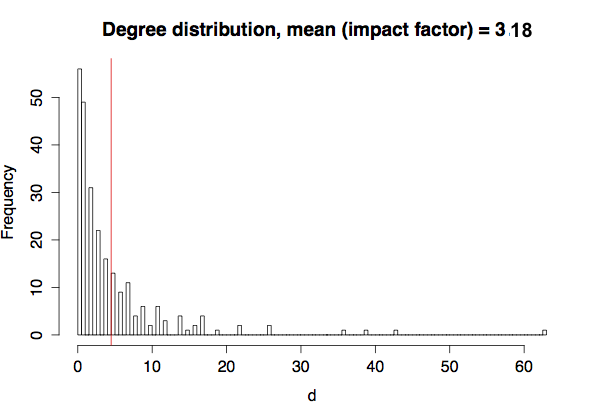
\includegraphics[width=\textwidth]{figures/degreeDistrib.png}
\end{column}
\begin{column}{0.25\textwidth}
\footnotesize
\justify
\textit{The stationary integrated impact factor, estimated as average citation count, means that a cybergeo paper gets at least 3 citations in its lifetime}
\end{column}
\end{columns}



\end{frame}


\jframe{Citation Network Structure}{

\centering
\includegraphics[height=0.75\textheight]{figures/citnw}

}



\begin{frame}
\frametitle{Hierarchy in citations}
\begin{columns}
\begin{column}{0.8\textwidth}
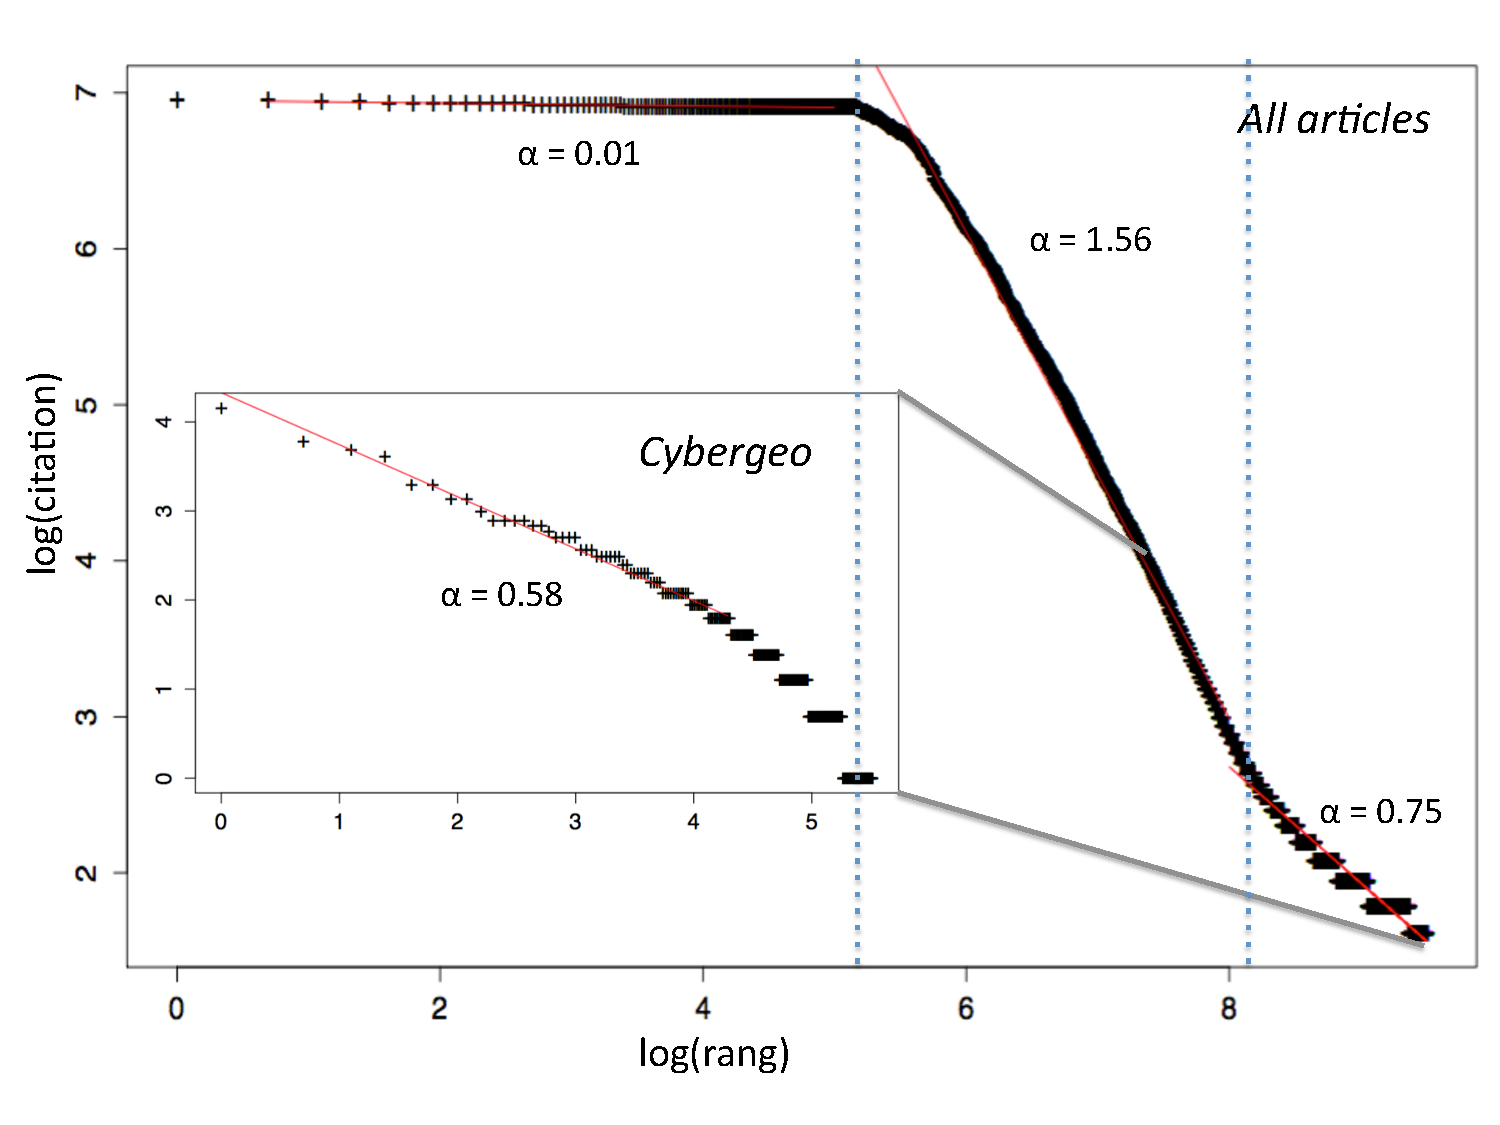
\includegraphics[width=\textwidth]{figures/ranksize.pdf}
\end{column}
\begin{column}{0.2\textwidth}
\justify
\textit{Superposition of different hierarchical citation regimes}
\end{column}
\end{columns}

\end{frame}




\jframe{Cliques}{
\textit{Complete subgraphs reveal strong affiliation patterns}
%\vspace{-1cm}
%\hspace{-2.3cm}

\bigskip

\centering

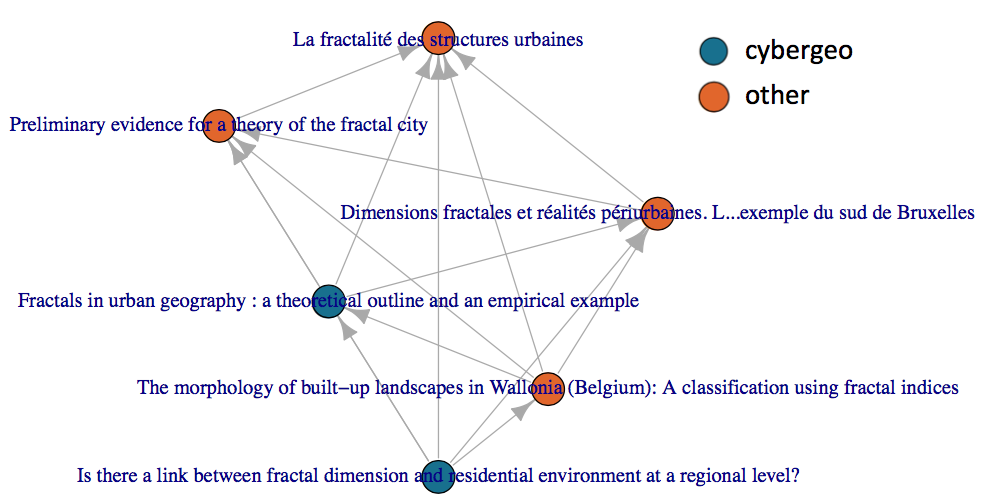
\includegraphics[width=\textwidth]{figures/cybclic.png}

}







\subsection{Semantic Network}


\jframe{Semantic Network}{


\textbf{Semantic Data : } Collection of abstract/date/authors/keywords for the 400000 references via Mendeley API
$\rightarrow$ $\sim 215000$ references with full data.

\bigskip

\textbf{Summary Statistics}

\textit{Language :} English 206607, French 4109, Spanish 2029, German 892, Portuguese 891, Dutch 124, others 182

\bigskip
\bigskip

\textit{Yearly count}
\centering

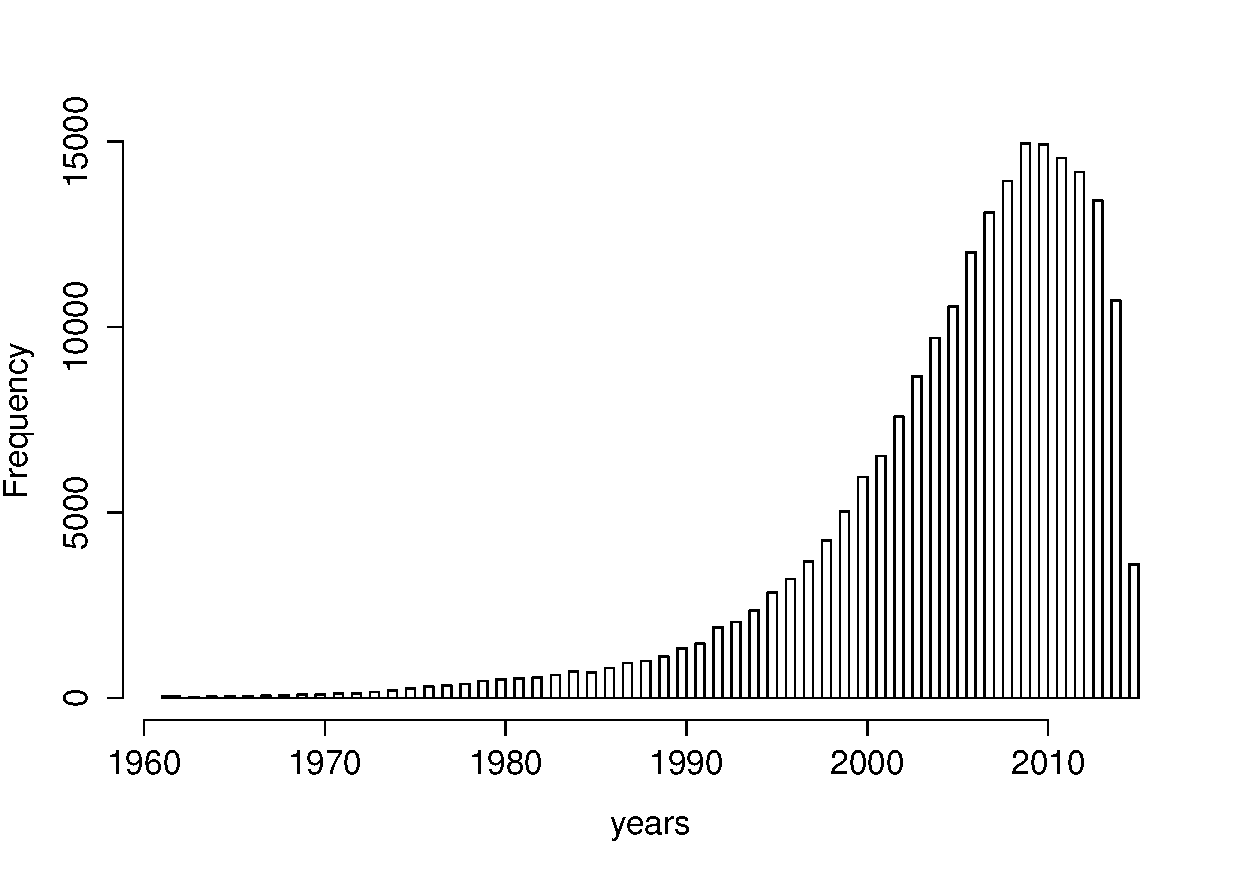
\includegraphics[width=0.4\textwidth,height=0.4\textheight]{figures/years}

}



\jframe{Keywords Extraction}{

%\textit{Text-mining en python avec \texttt{nltk}~\cite{bird2006nltk}}, m{\'e}thode adapt{\'e}e de
%\cite{chavalarias2013phylomemetic}

\textit{Text-mining in python with \texttt{nltk}~\cite{bird2006nltk}}, method adpated from
\cite{chavalarias2013phylomemetic}


\bigskip

\begin{itemize}
\item Language detection using \textit{stop-words}
\item Parsing and tokenizing / pos-tagging (word functions) / stemming done differently depending on language :
\begin{itemize}
\item English : \texttt{nltk} built-in pos-tagger, combined to a \emph{PorterStemmer}
\item French or other : use of \texttt{TreeTagger}~\cite{schmid1994probabilistic}
\end{itemize}
\item Selection of potential \textit{n-grams} (with $1 \leq n \leq 4$) : English $\bigcap \{NN \cup VBG \cup JJ \}$ ;  French  $\bigcap \{NOM \cup ADJ\}$
\item Database insertion for instantaneous utilisation (10j $\rightarrow$ 2min)
\item Estimation of \textit{n-grams} relevance, following co-occurrences statistical distribution
\end{itemize}


}




\jframe{Construction of Semantic Network}{

\begin{itemize}

%\item \textbf{Noeuds :} Mots-cl{\'e}s avec la plus grande pertinence cumul{\'e}e

\item \textbf{Nodes :} Keywords with largest relevance


\medskip

\item \textbf{Links :} Weighted co-occurrences

\medskip

\item Manual suppression of parasite words (e.g. : copyright statements !)

\medskip

\item Low weight link filtering

\medskip

\item Suppression of \textit{hubs} (ex. \texttt{model}, \texttt{space}, \texttt{structure}, \texttt{process}) that suppress community structure

\item Community detection by greedy modularity maximization (Louvain method~\cite{blondel2008fast})

\medskip 

\end{itemize}


}


\begin{frame}
\frametitle{Parameters influence}
\textit{Importance of \textbf{fine tuning} : }

$\rightarrow$ Sensitivity of models \textbf{and} data analysis to parameters. Systematic exploration mandatory, via OpenMole for example.

$\rightarrow$ Place of expert decision-making : no qualitative-quantitative dichotomy

\medskip

\begin{columns}
\begin{column}{0.65\textwidth}
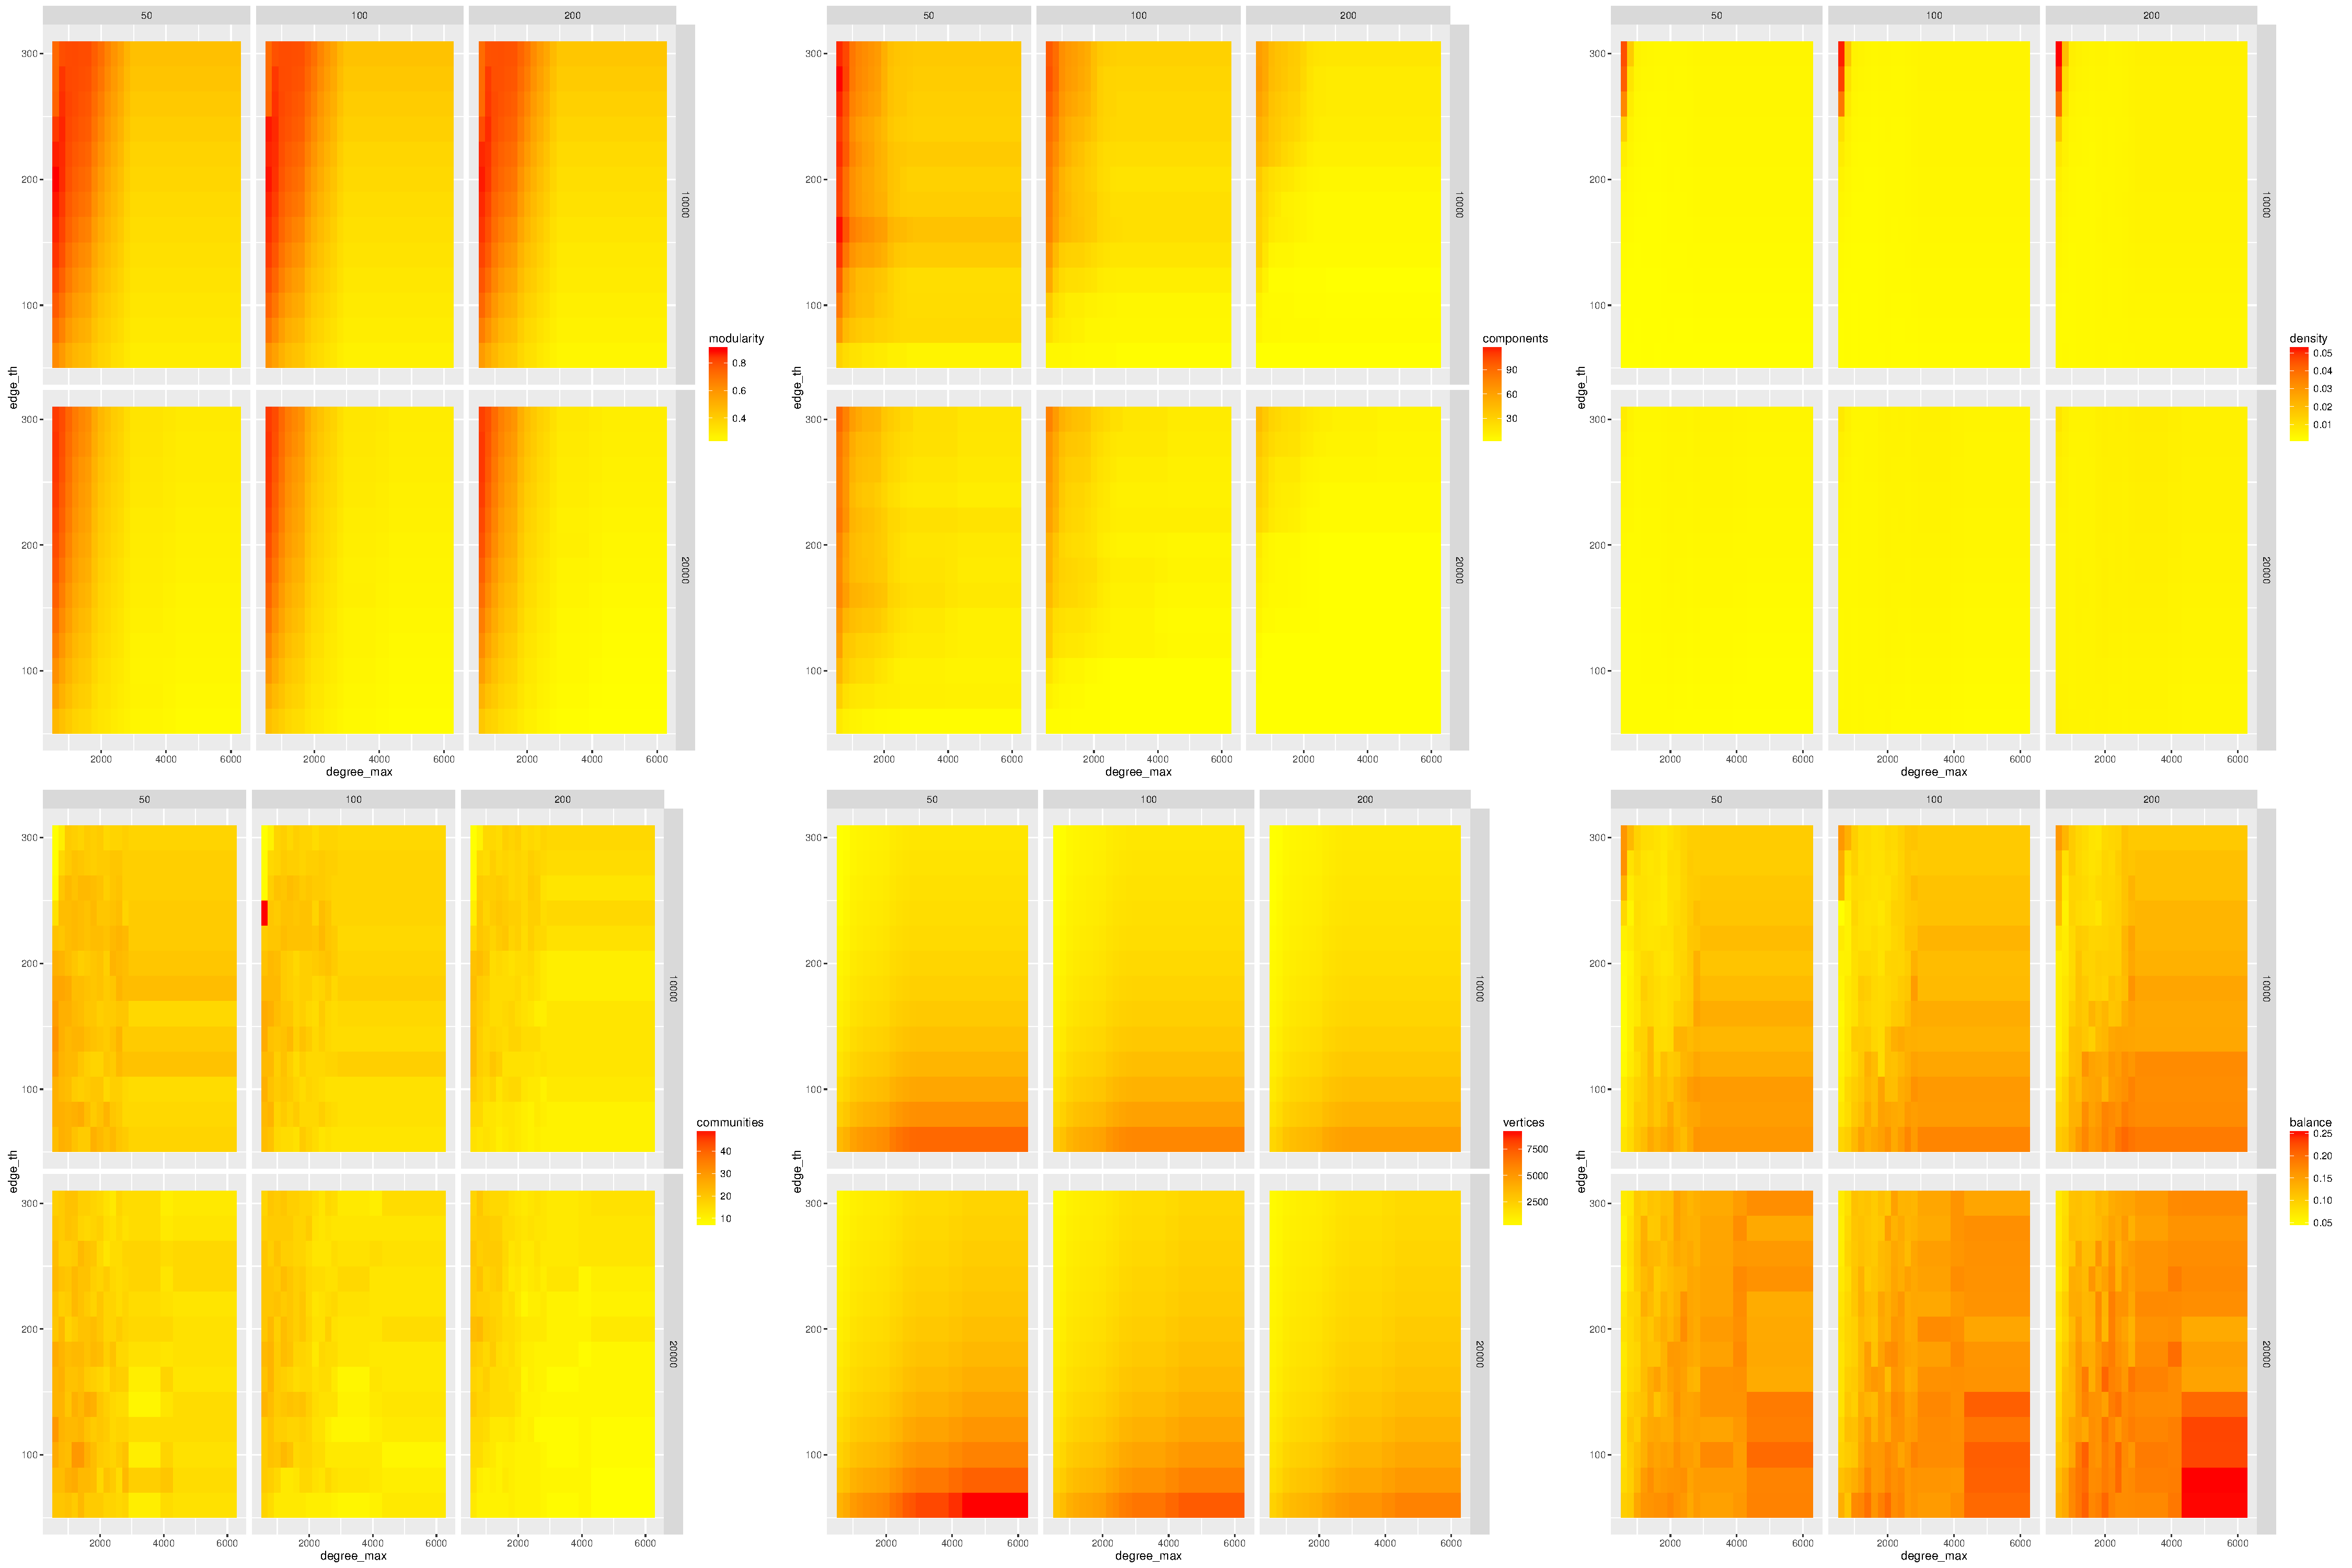
\includegraphics[width=\textwidth]{figures/sensitivity_facet_allindics}
\end{column}
\begin{column}{0.25\textwidth}
\justify
\textit{Multi-criteria optimization (modularity, size, balance) on network construction parameters}
\end{column}
\end{columns}
\end{frame}

%


\jframe{Obtained disciplines}{
\textit{Communities obtained with $\theta_V=1200,\theta_E=50$}
\bigskip
{\footnotesize
\begin{itemize}
\item Political sciences/critical geography (535) : \texttt{decision-mak, polit ideolog, democraci, stakehold, neoliber}
\item Biogeography (394) : \texttt{plant densiti, wood, wetland, riparian veget}
\item Economic geography (343) : \texttt{popul growth, transact cost, socio-econom, household incom}
\item Environnment/climate (309) : \texttt{ice sheet, stratospher, air pollut, climat model}
\item Complex systems (283) : \texttt{scale-fre, multifract, agent-bas model, self-organ}
\item Physical geography (203) : \texttt{sedimentari, digit elev model, geolog, river delta}
\item Spatial analysis (175) : \texttt{spatial analysi, princip compon analysi, heteroscedast, factor analysi}
\end{itemize}
}
}

\jframe{Obtained disciplines (continued)}{
{\footnotesize
\begin{itemize}
\item Microbiology (118) : \texttt{chromosom, phylogenet, borrelia}
\item Statistical methods (88) : \texttt{logist regress, classifi, kalman filter, sampl size}
\item Cognitive sciences (81) : \texttt{semant memori, retrospect, neuroimag}
\item GIS (75) : \texttt{geograph inform scienc, softwar design, volunt geograph inform, spatial decis support}
\item Traffic modeling (63) : \texttt{simul model, lane chang, traffic flow, crowd behavior}
\item Health (52) : \texttt{epidem, vaccin strategi, acut respiratori syndrom, hospit}
\item Remote sensing (48) : \texttt{land-cov, landsat imag, lulc}
\item Crime (17) : \texttt{crimin justic system, social disorgan, crime}
\end{itemize}

}
}

\begin{frame}
\frametitle{Network}
\begin{columns}
  \begin{column}{0.6\textwidth}
    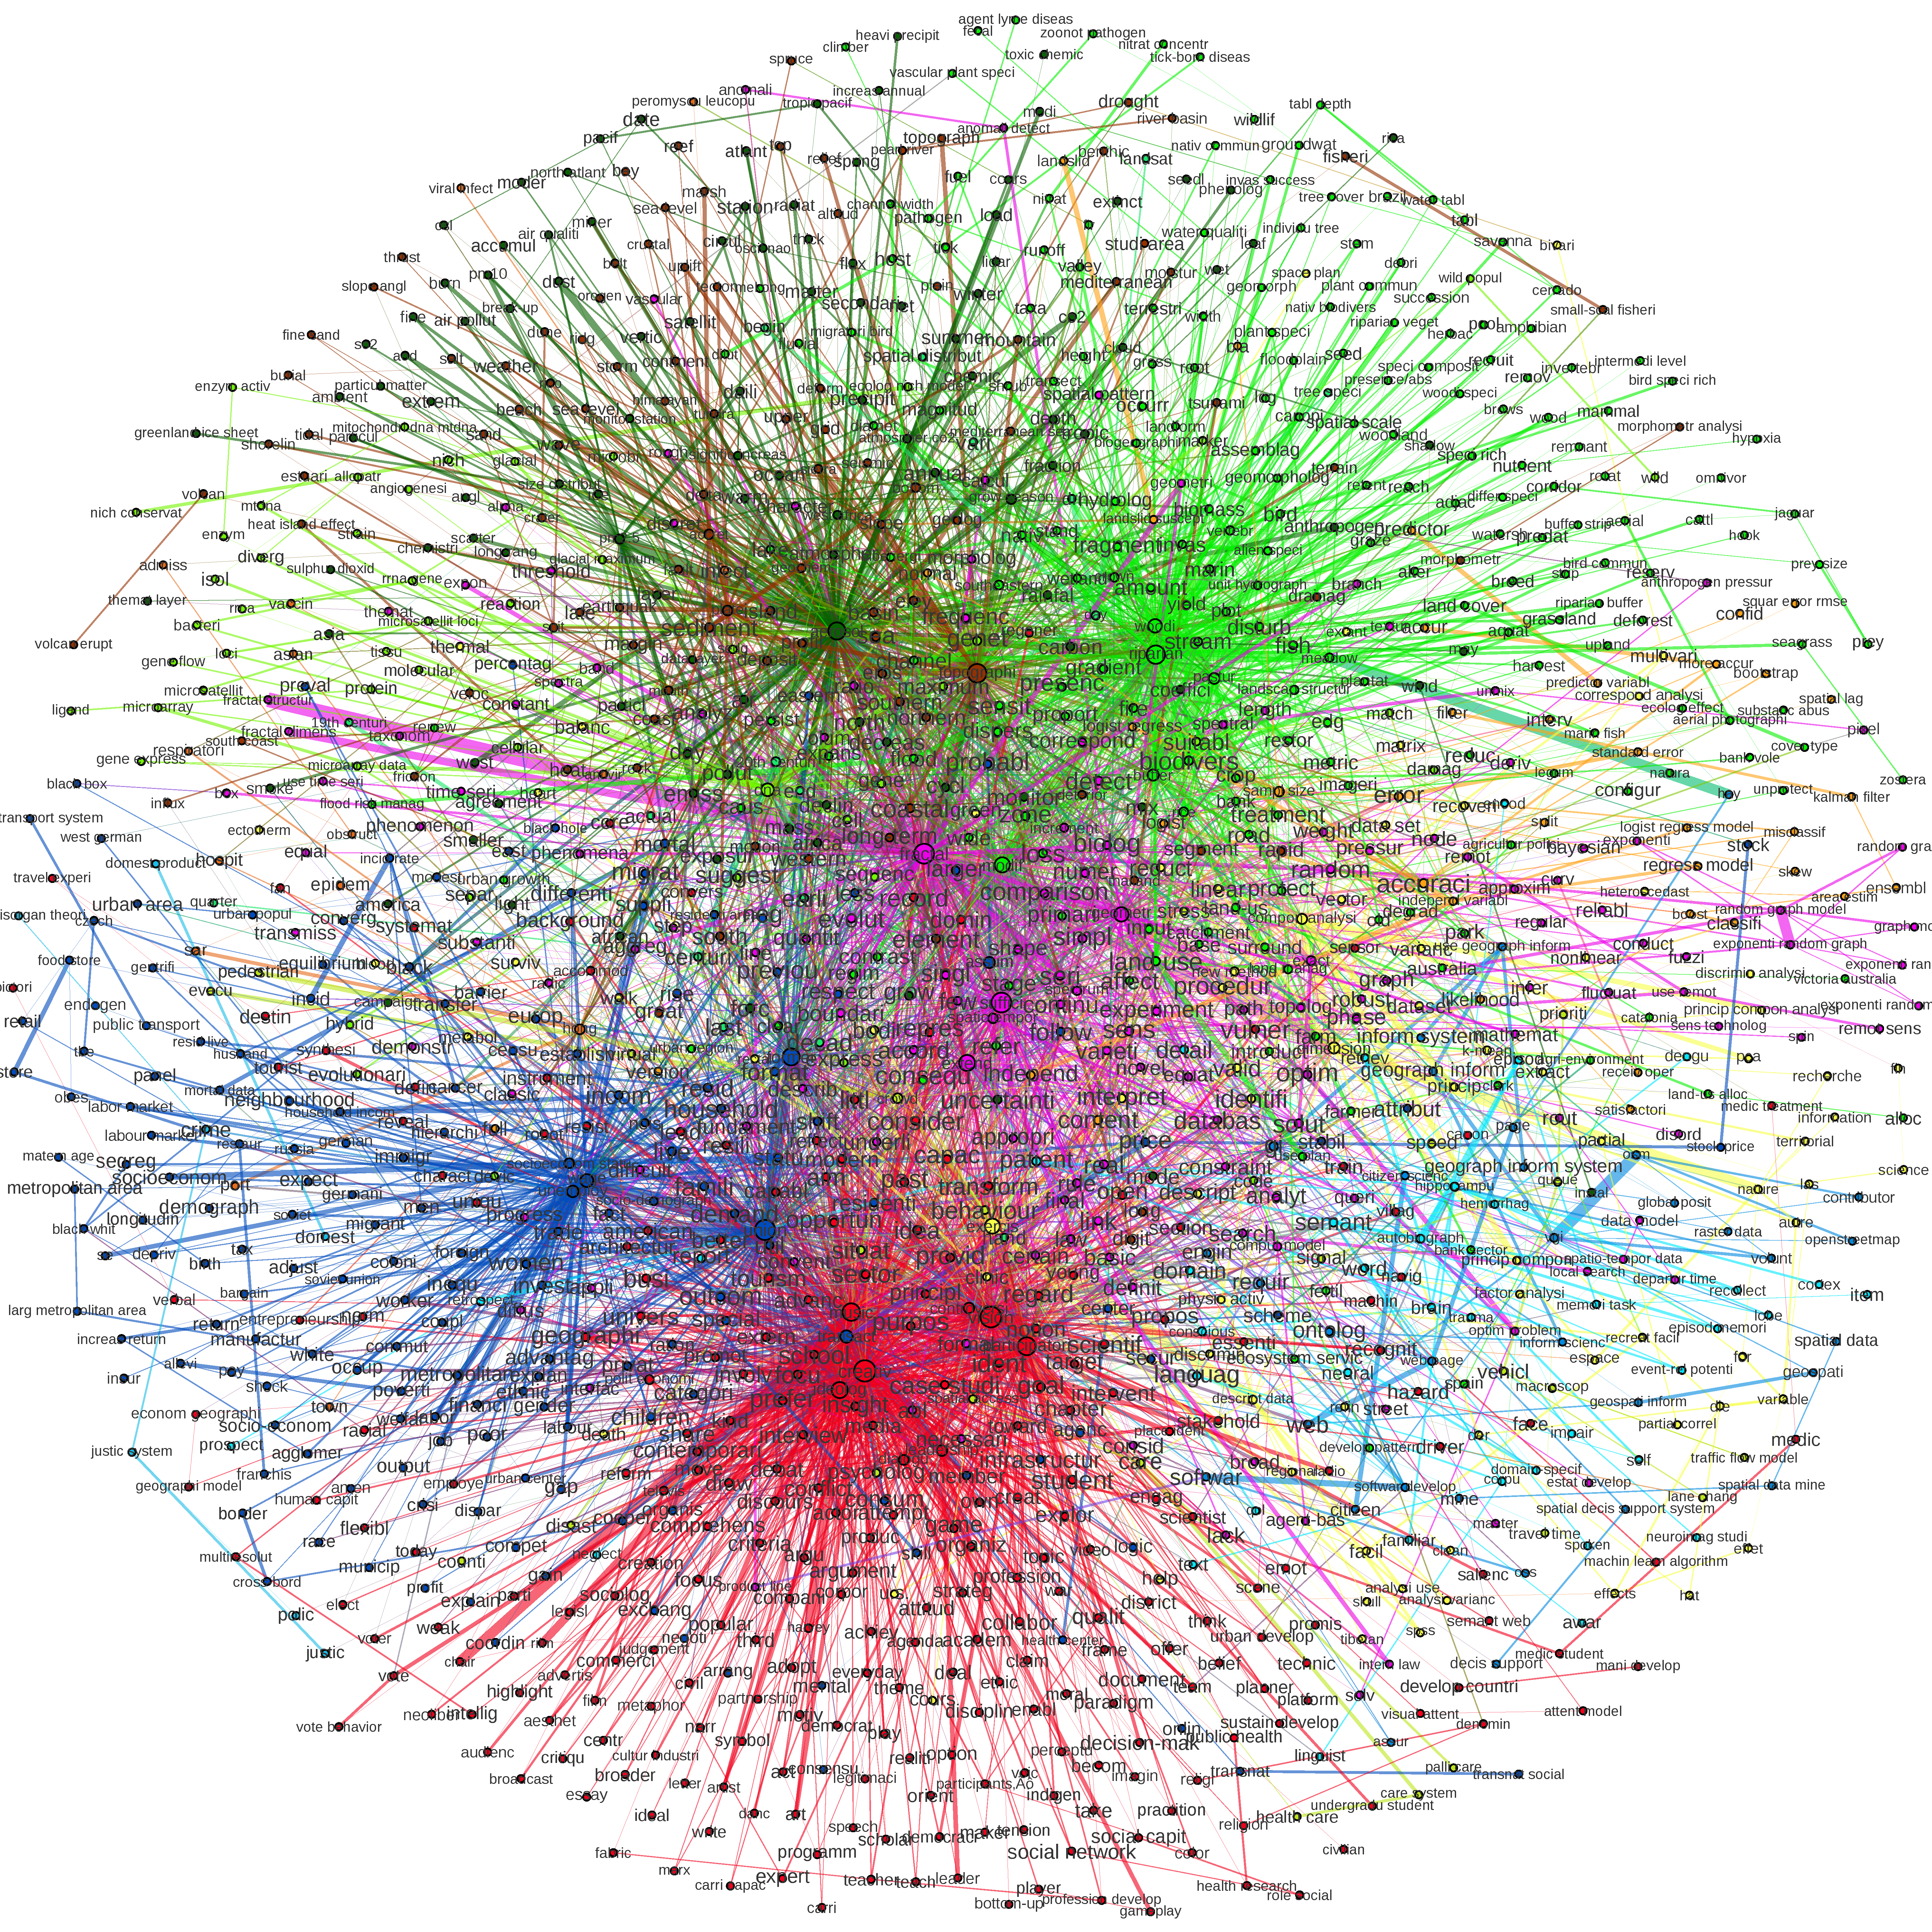
\includegraphics[height=0.74\textheight]{figures/semantic.png}
  \end{column}
  \begin{column}{0.4\textwidth}
    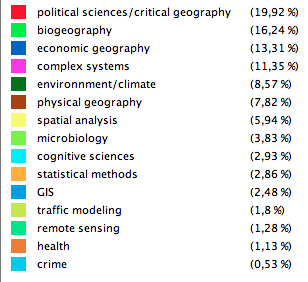
\includegraphics[width=\textwidth]{figures/disciplines.png}
  \end{column}
\end{columns}
\end{frame}


\begin{frame}
\frametitle{Interdisicplinarity}

\begin{columns}
\begin{column}{0.6\textwidth}
%\vspace{-0.2cm}
\includegraphics[width=\textwidth]{figures/synththemcyb}
\end{column}
\begin{column}{0.4\textwidth}
\justify
\textit{Synthetic representation of disciplines. Link strength gives the probability for two disciplines to jointly appear in a paper}
\end{column}
\end{columns}



\end{frame}




\begin{frame}
\frametitle{Citation interdisicplinarity}

\begin{columns}
\begin{column}{0.6\textwidth}
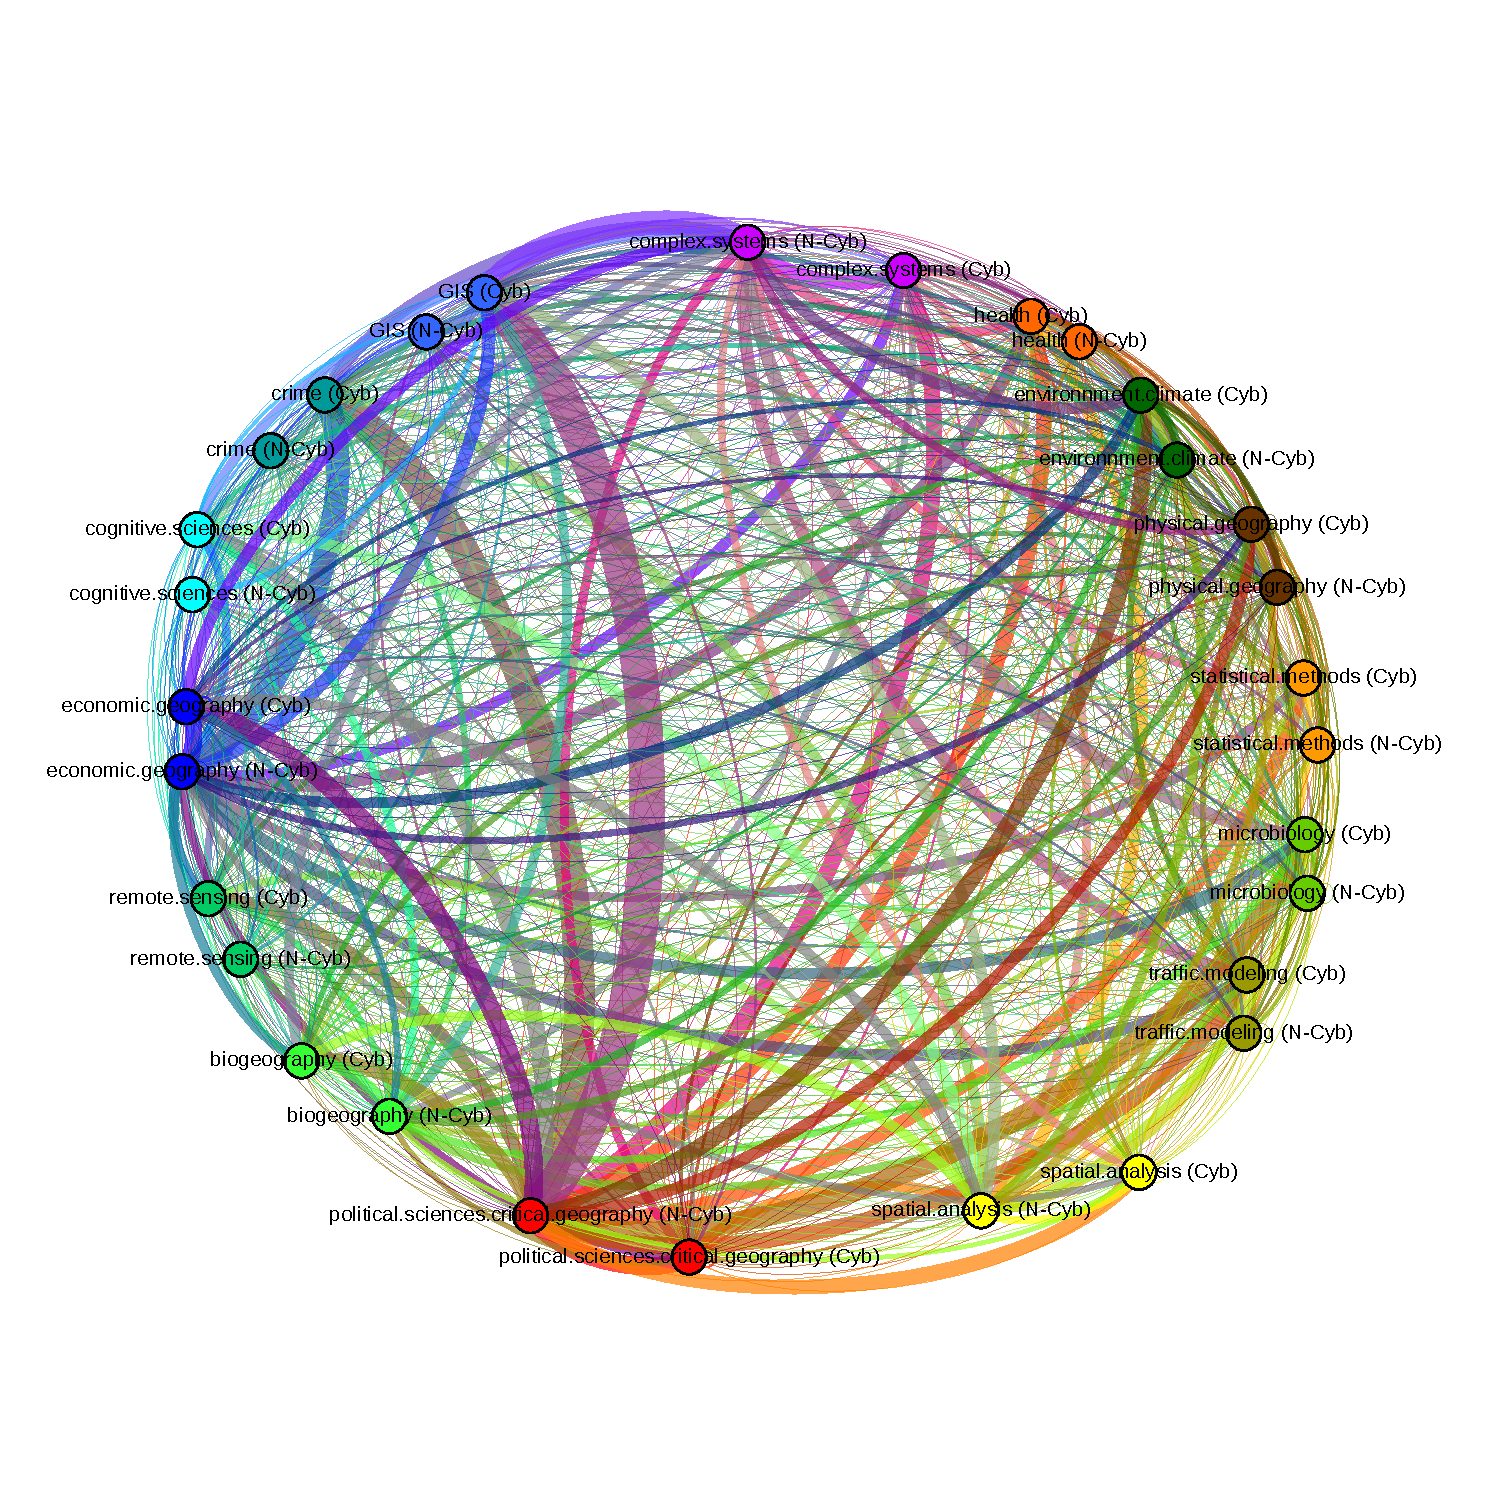
\includegraphics[height=0.9\textheight]{figures/citation}
\end{column}
\begin{column}{0.05\textwidth}
\end{column}
\begin{column}{0.25\textwidth}
\justify
\textit{Citation flows between disciplines (directed links to be read in anti-trigonometric sense) reveal citation level interdisciplinarity}
\end{column}
\end{columns}
\end{frame}




\begin{frame}
\frametitle{Article-level interdisciplinarity}

%Un article peut {\^e}tre associ{\'e} aux communaut{\'e}s s{\'e}mantiques par ses mots cl{\'e}s : probas $p_i$ pour chaque communaut{\'e}.

%Mesure d'interdisciplinarit{\'e} (pour un article, au premier ordre) :
%\[
%o = 1 - \sum p_i^2
%\]

\begin{columns}
\begin{column}{0.7\textwidth}
An article has a proportion of keywords in each discipline, which can be understood as probabilities $(p_i)$. Interdisciplinarity index defined as $i = 1 - \sum p_i^2$.

\bigskip

\centering

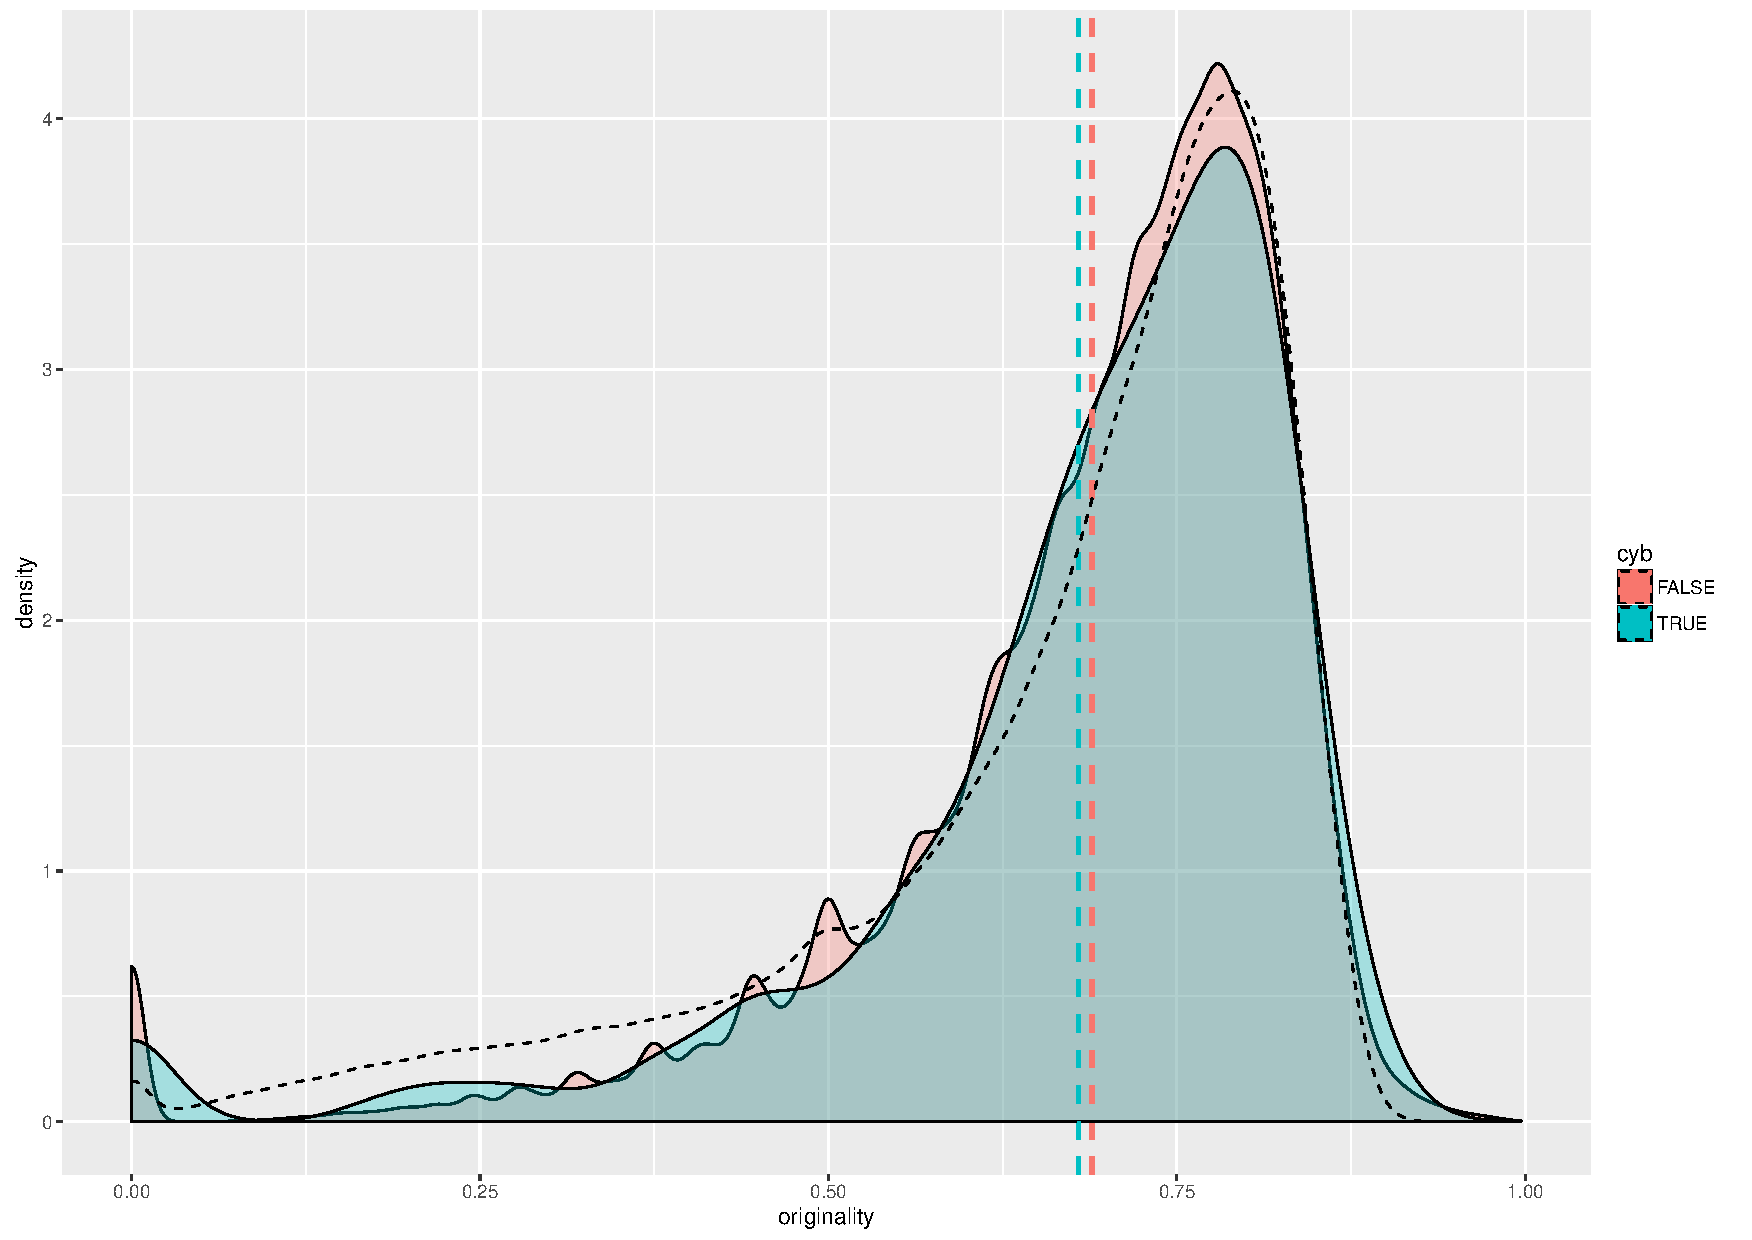
\includegraphics[width=0.8\textwidth]{figures/firstorderint_withNull}

\end{column}
\begin{column}{0.3\textwidth}
\vspace{-1cm}
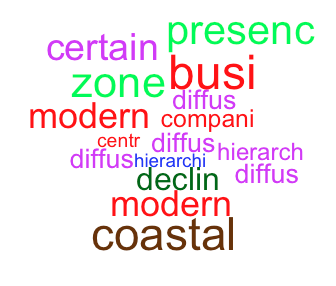
\includegraphics[width=\textwidth]{figures/exampleWordcloud_24872}
\vspace{1cm}
\textit{Distribution of article interdisciplinarities (null model in dotted line). }
\end{column}
\end{columns}

\end{frame}


\begin{frame}
\frametitle{Citation interdisciplinarity}

\textit{Citation interdisciplinarity defined the same way, based on probabilities to cite or be cited by a discipline.}

\bigskip

\begin{columns}
\begin{column}{0.5\textwidth}
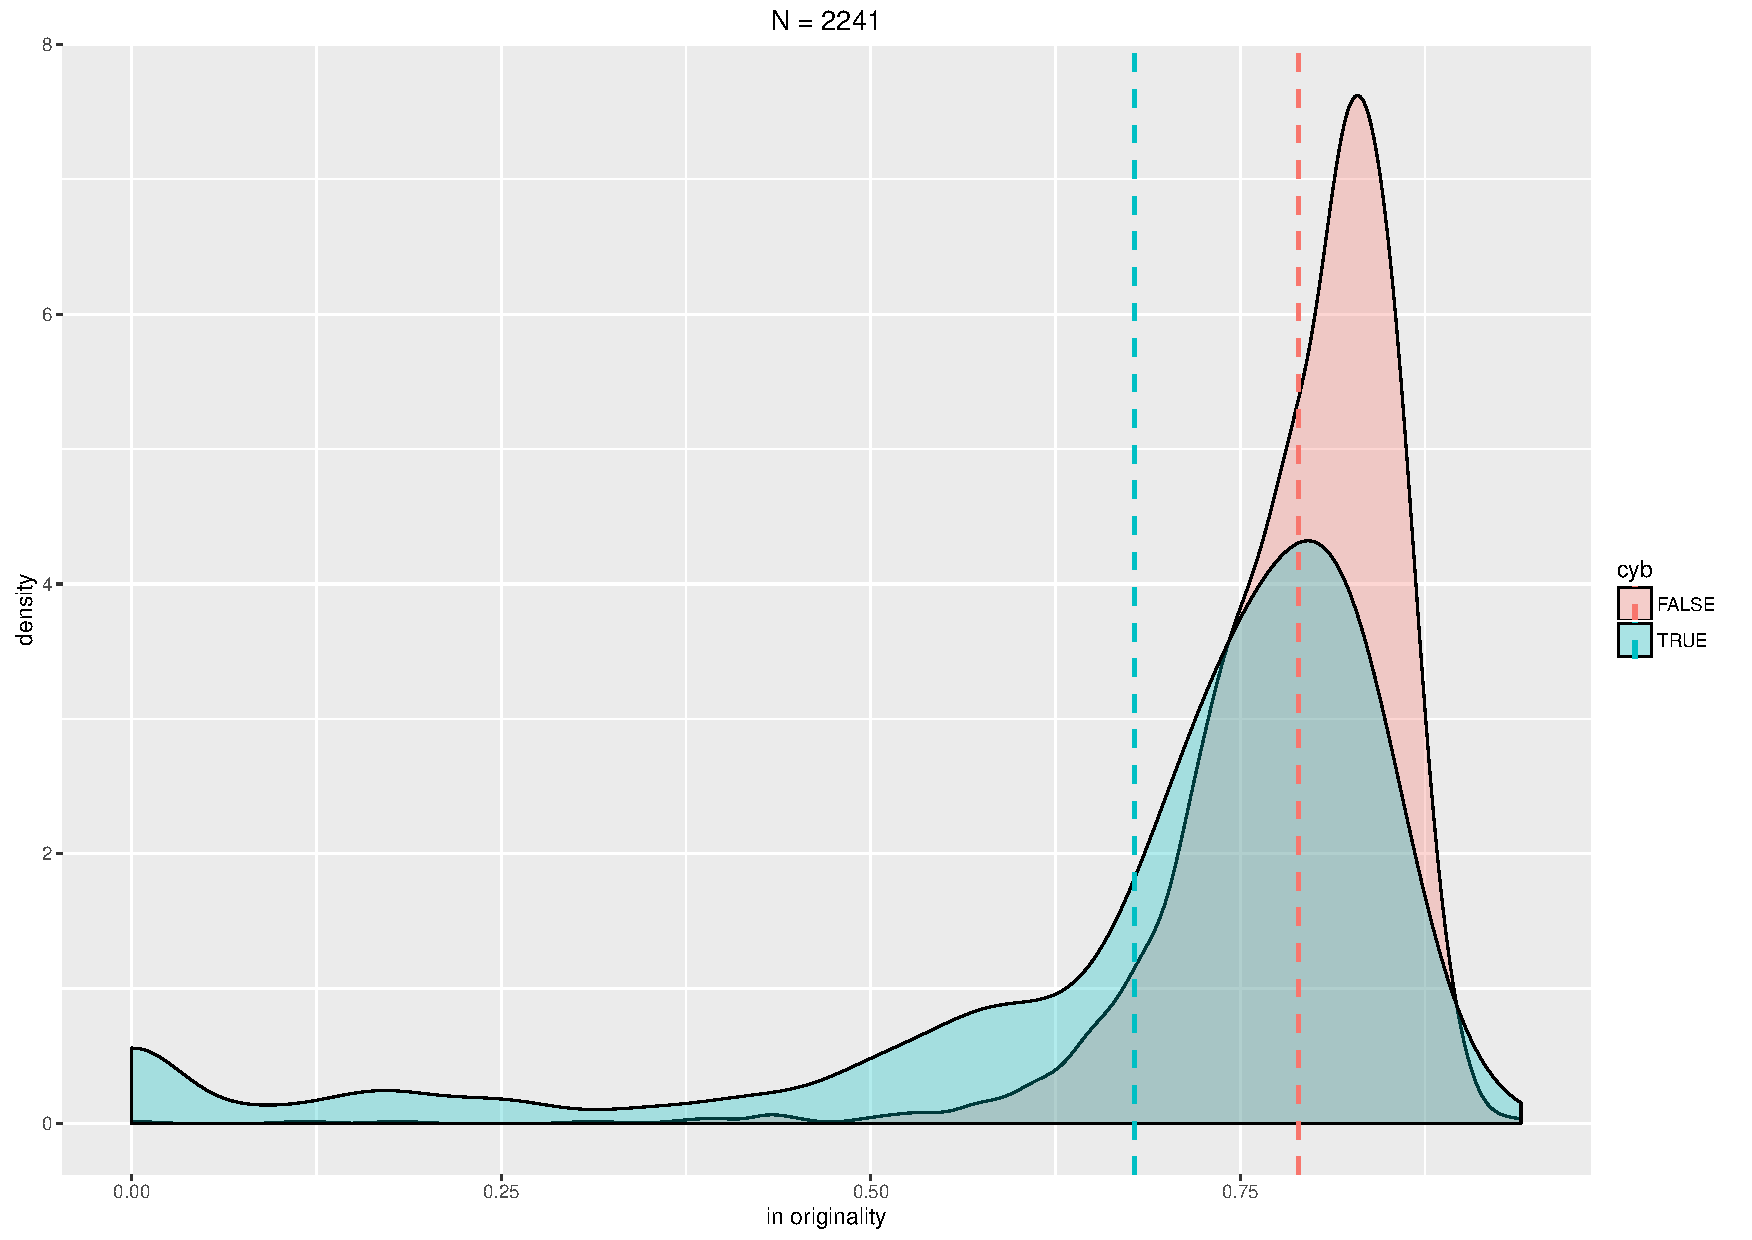
\includegraphics[width=\textwidth]{figures/citin_interdisc}

\textit{Citing article interdisciplinarity distribution. Cybergeo papers are cited by less different disciplines, what can be explained by their young age.}
\end{column}
\begin{column}{0.5\textwidth}
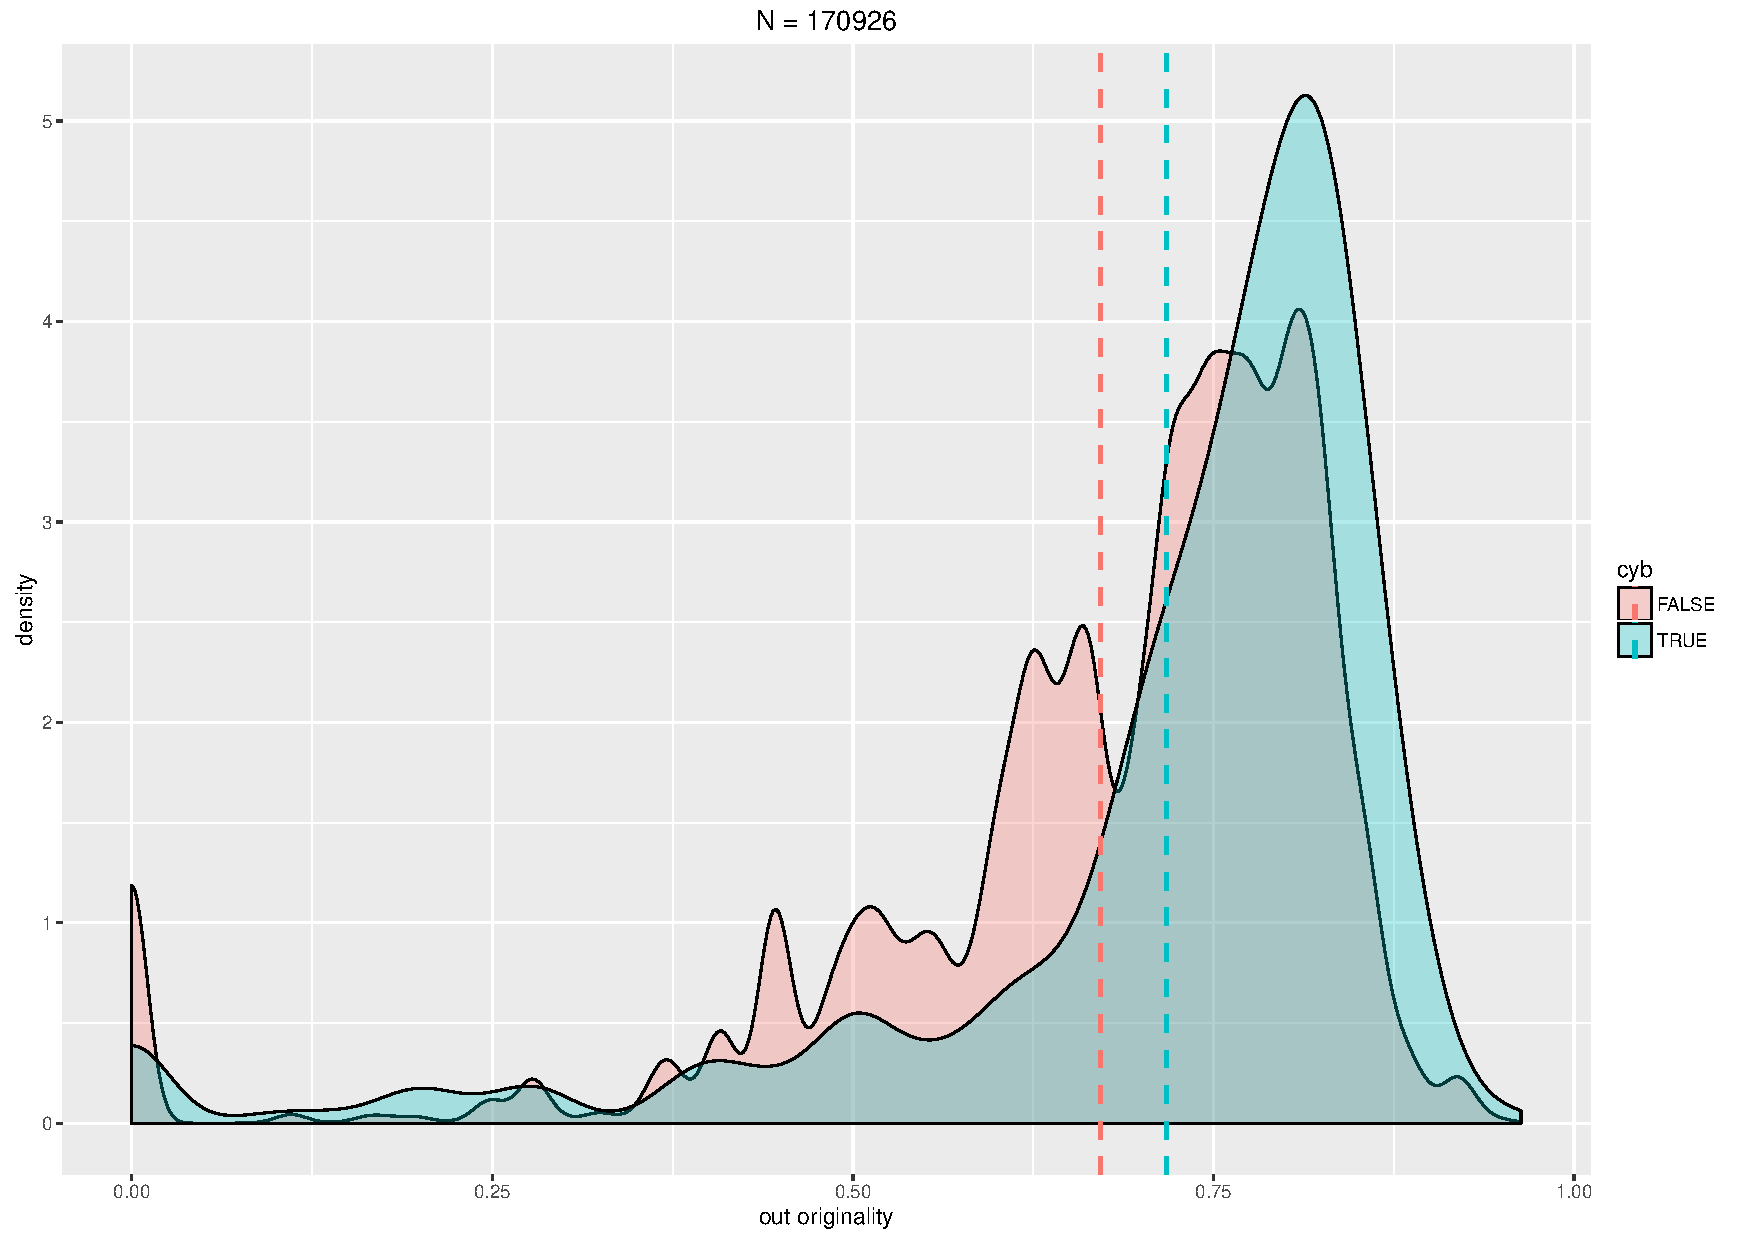
\includegraphics[width=\textwidth]{figures/citout_interdisc}

\textit{Cited article interdisciplinarity distribution. Distribution for all articles is directly shaped by citation network structure.}
\end{column}
\end{columns}
\end{frame}


\begin{frame}
\frametitle{Interactive exploration}
\textit{On \texttt{CybergeoNetworks} : Article level citation and semantic exploration ; semantic network exploration}

\bigskip
\bigskip


\begin{columns}
\begin{column}{0.45\textwidth}
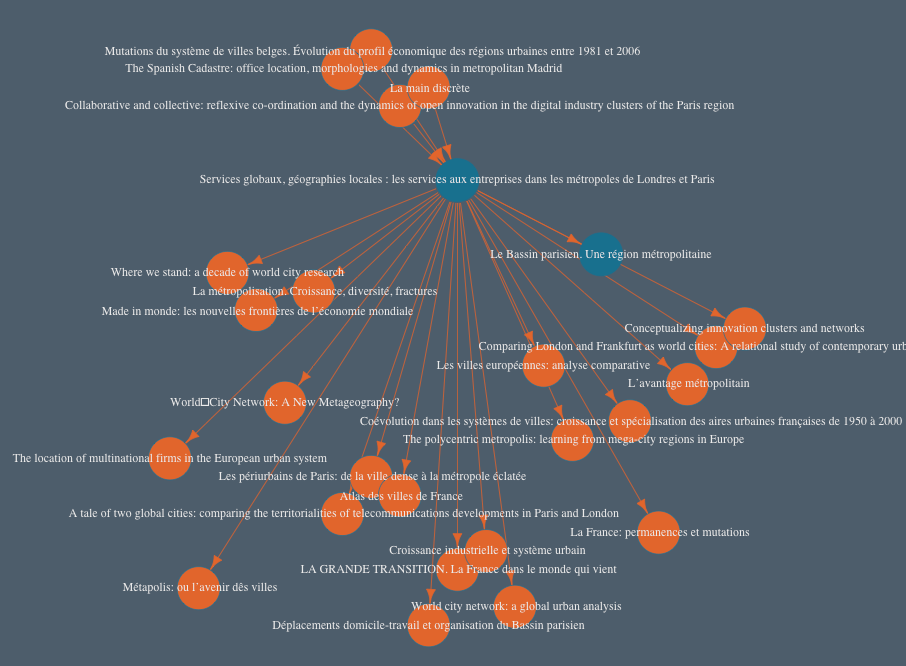
\includegraphics[width=\textwidth]{figures/ex_citvisu_23337}
\end{column}
\begin{column}{0.55\textwidth}
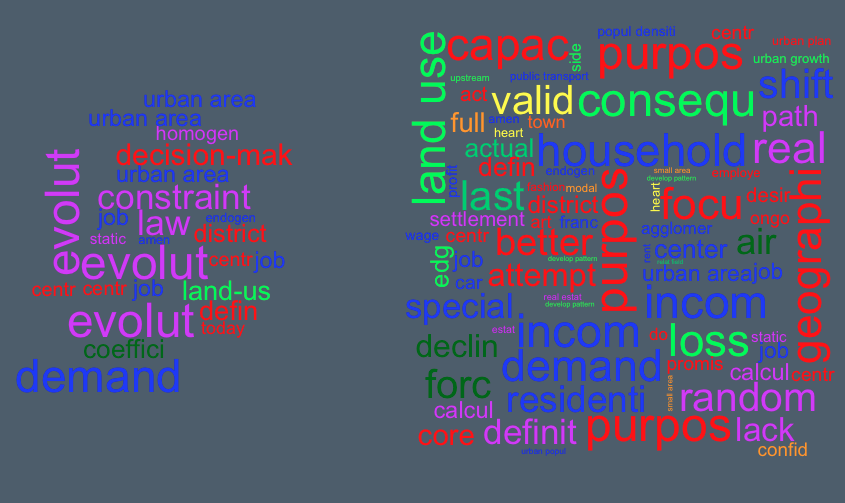
\includegraphics[width=\textwidth]{figures/ex_visuwordcloud_25892}
\end{column}
\end{columns}

\end{frame}




\jframe{Conclusion}{
  %$\rightarrow$ Un environnement disciplinaire tr{\`e}s vari{\'e} et une interdicisplinarit{\'e} affirm{\'e}e
  
  $\rightarrow$ A very rich scientific environment and a confirmed interdisciplinarity
  
  \bigskip
  
  %$\rightarrow$ Approche {\`a} croiser avec autres types de classifications (th{\'e}matique (POC), mots-cl{\'e}s (HC), g{\'e}ographique (CC) pour en apprendre plus sur la revue et la pratique de la g{\'e}ographie qui lui est associ{\'e}e
  
  $\rightarrow$ Approach to be combined with other classifications (thematic (POC), keywords (HC), geographical (CC)) to unveil patterns in geographical practices around the journal
  
  \bigskip
  
  %$\rightarrow$ M{\'e}thode g{\'e}n{\'e}rique pouvant s'appliquer {\`a} tout r{\'e}seau dont les noeuds ont une description textuelle
  
  $\rightarrow$ Generic method that can be applied to any network whose nodes have a textual description
  
}





\jframe{Reserve Slides}{
\Large \textit{Reserve Slides}
}





\jframe{Data Collection}{
\textit{Crawling of semi-open data : examples in geography}

\bigskip

%Donn{\'e}es de mobilit{\'e} : statuts des stations Vlib en temps r{\'e}el (API)

Mobility data : bike-sharing docking stations status (API)

\cite{raimbault2015user}

\bigskip

\centering
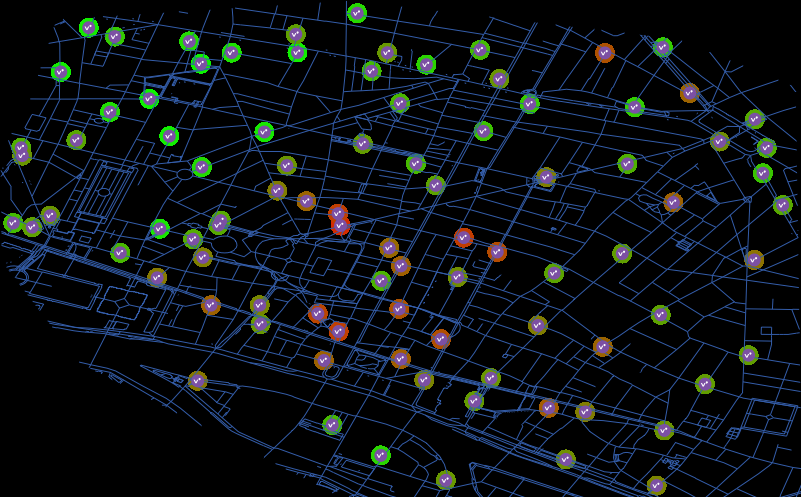
\includegraphics[width=0.7\textwidth]{figures/velib}



}

\jframe{Data Collection}{
\textit{Exemples in geography (continued)}

\bigskip

Road traffic : collect of \textit{sytadin} data (no API : \textit{scrapping} is necessary)


\bigskip

\centering
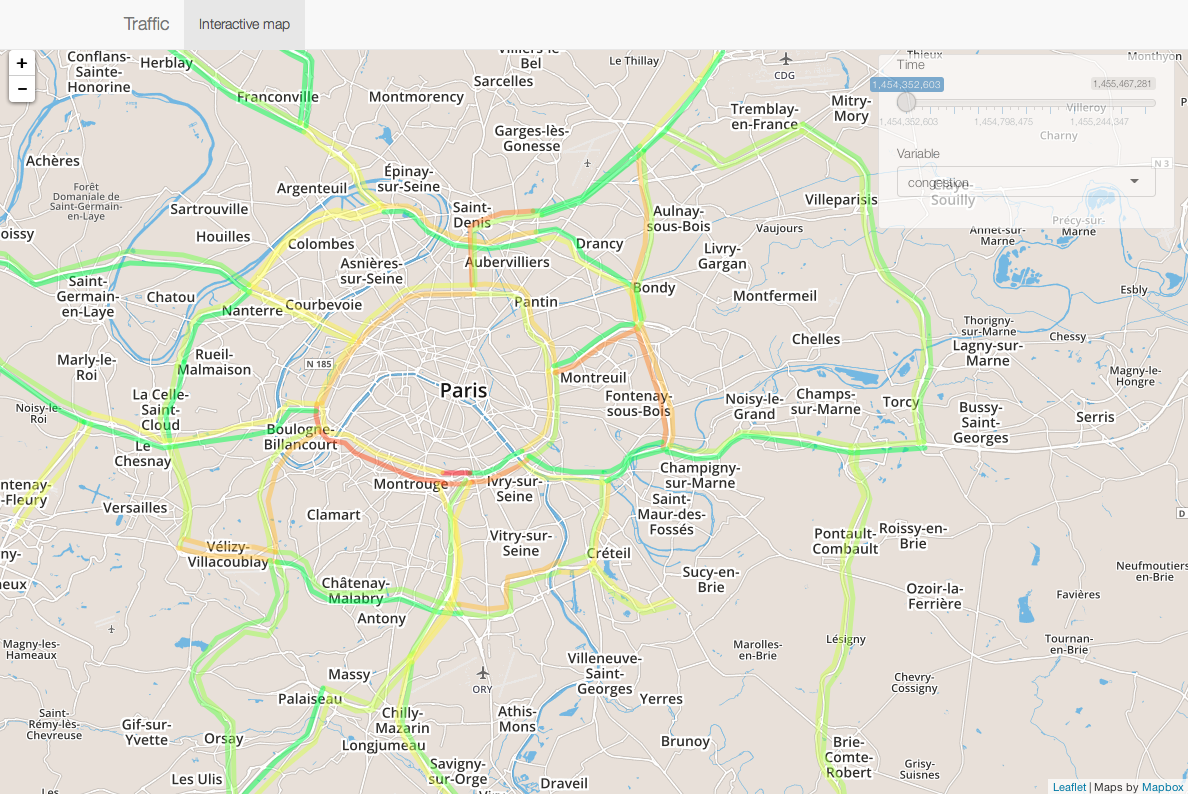
\includegraphics[width=0.8\textwidth]{figures/screen_appli}


\bigskip



}






\jframe{Centrality (citation)}{

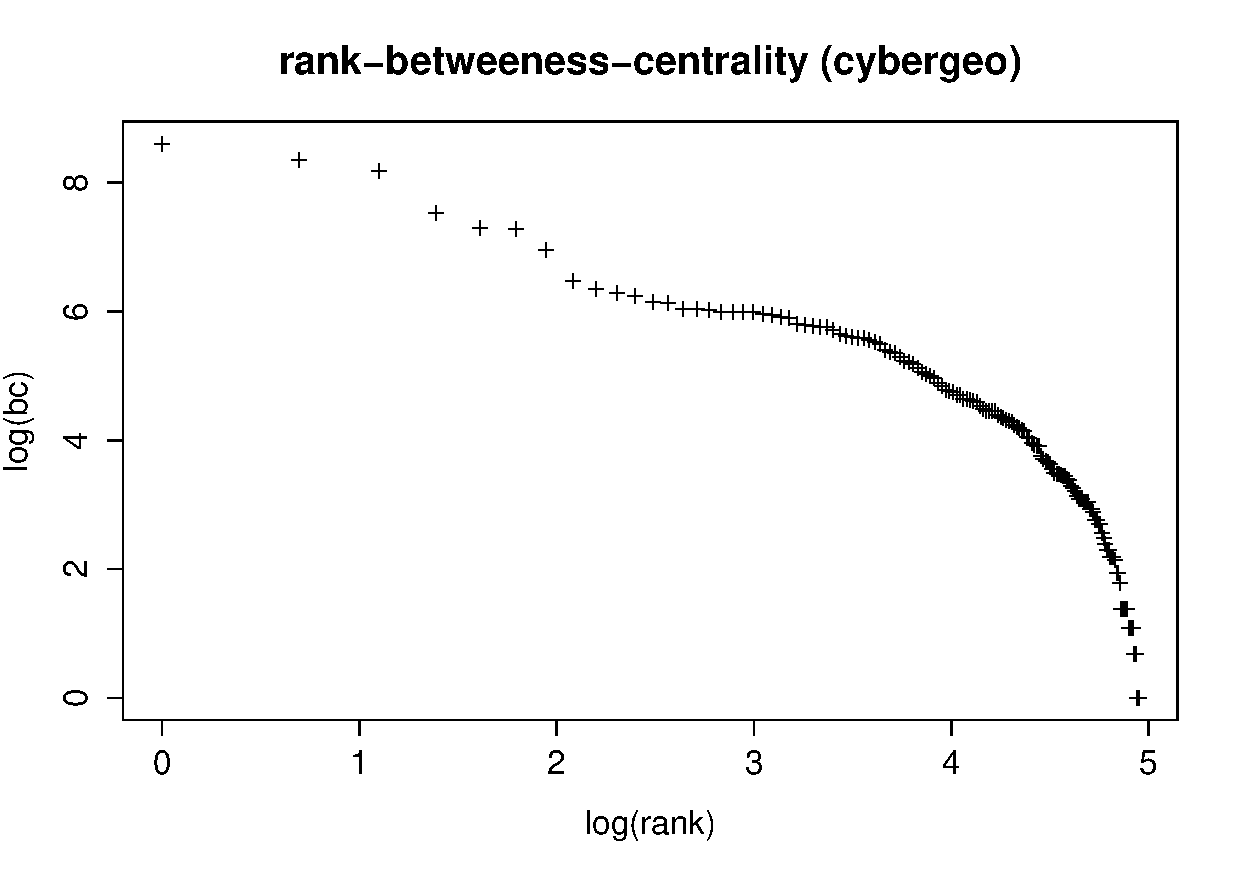
\includegraphics[width=0.5\textwidth]{figures/betweeness-cyb}
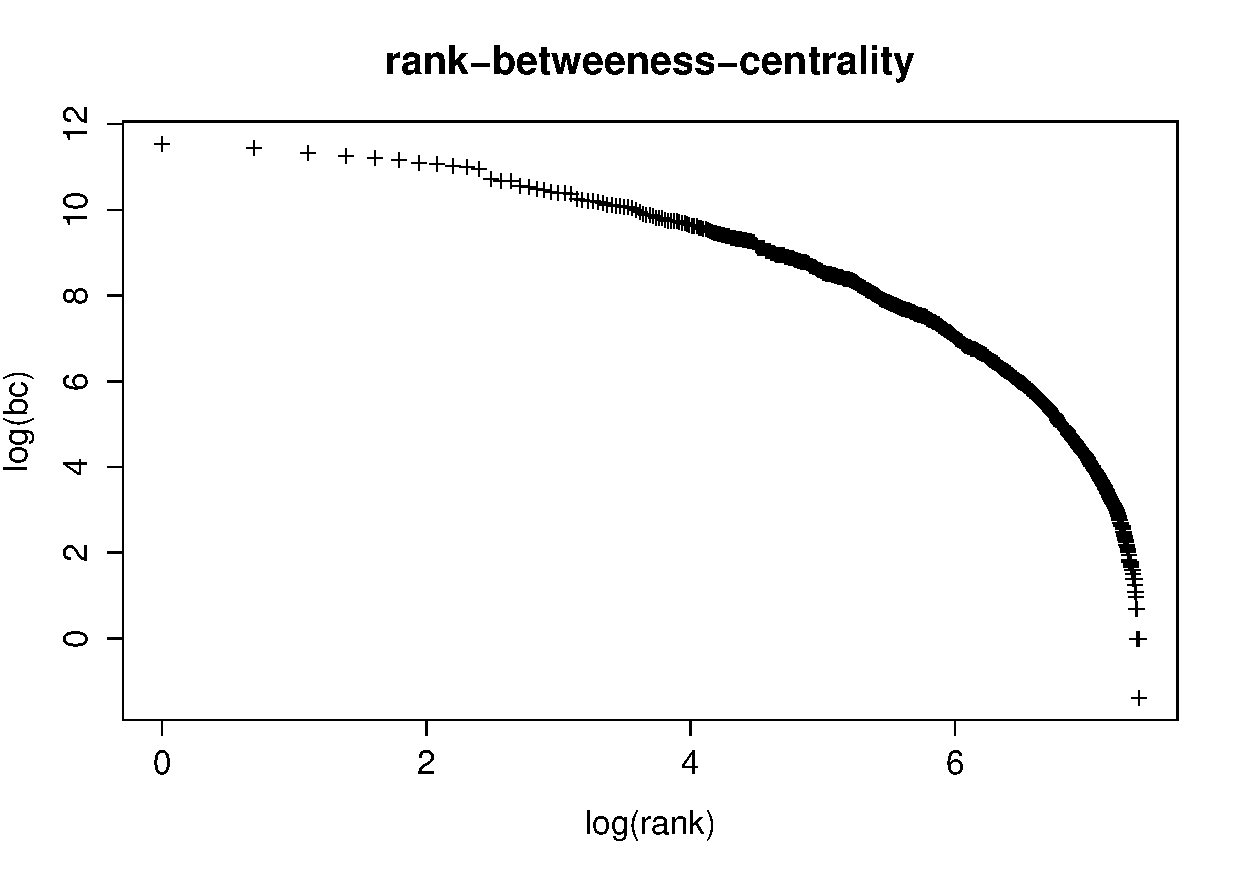
\includegraphics[width=0.5\textwidth]{figures/betweeness}

\textit{Weak centralities (rq : impossibility of having strong clusters because of temporal causality). Left : Cybergeo ; Right : Whole Network}

}


\jframe{Clustering (citation)}{
Giant component : more than 99\% of nodes.
\medskip

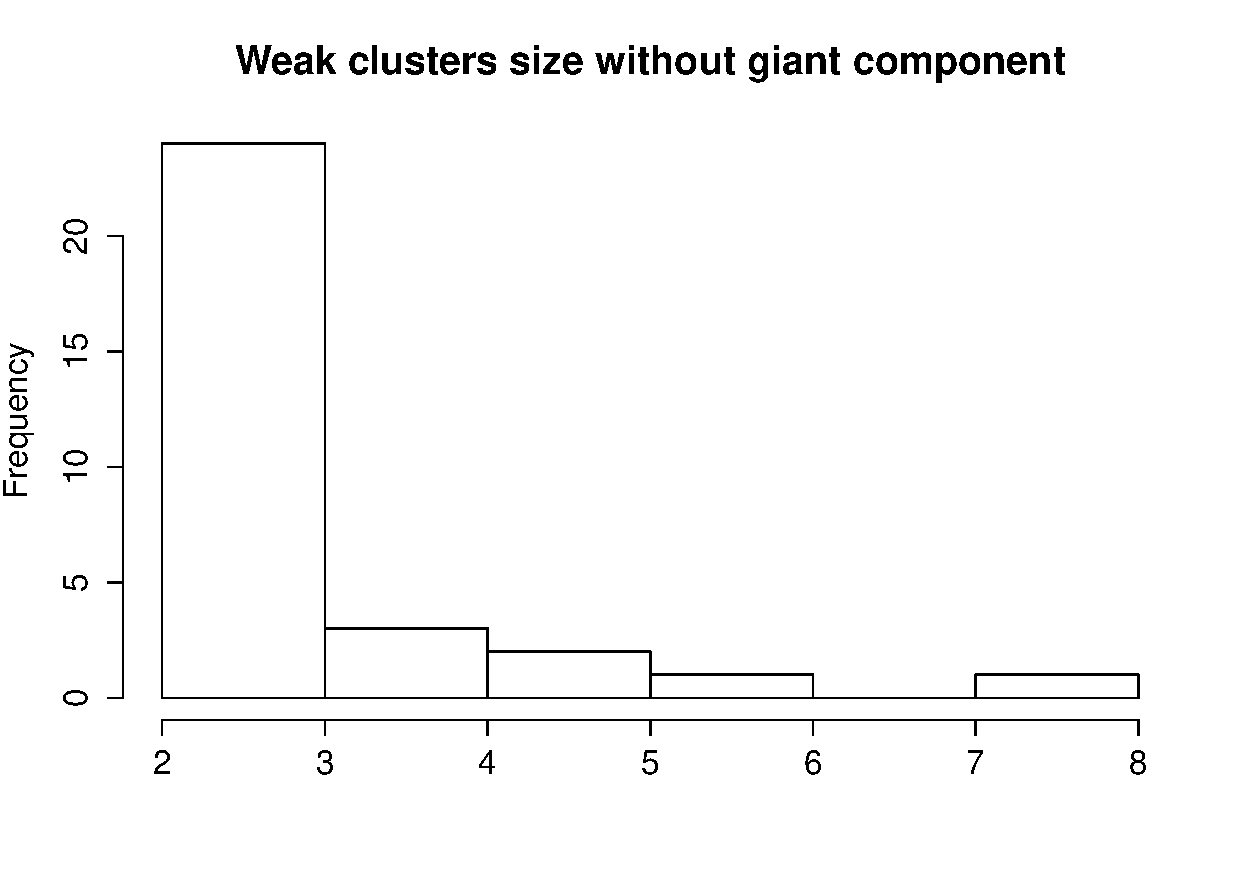
\includegraphics[width=0.5\textwidth]{figures/clusterSize}
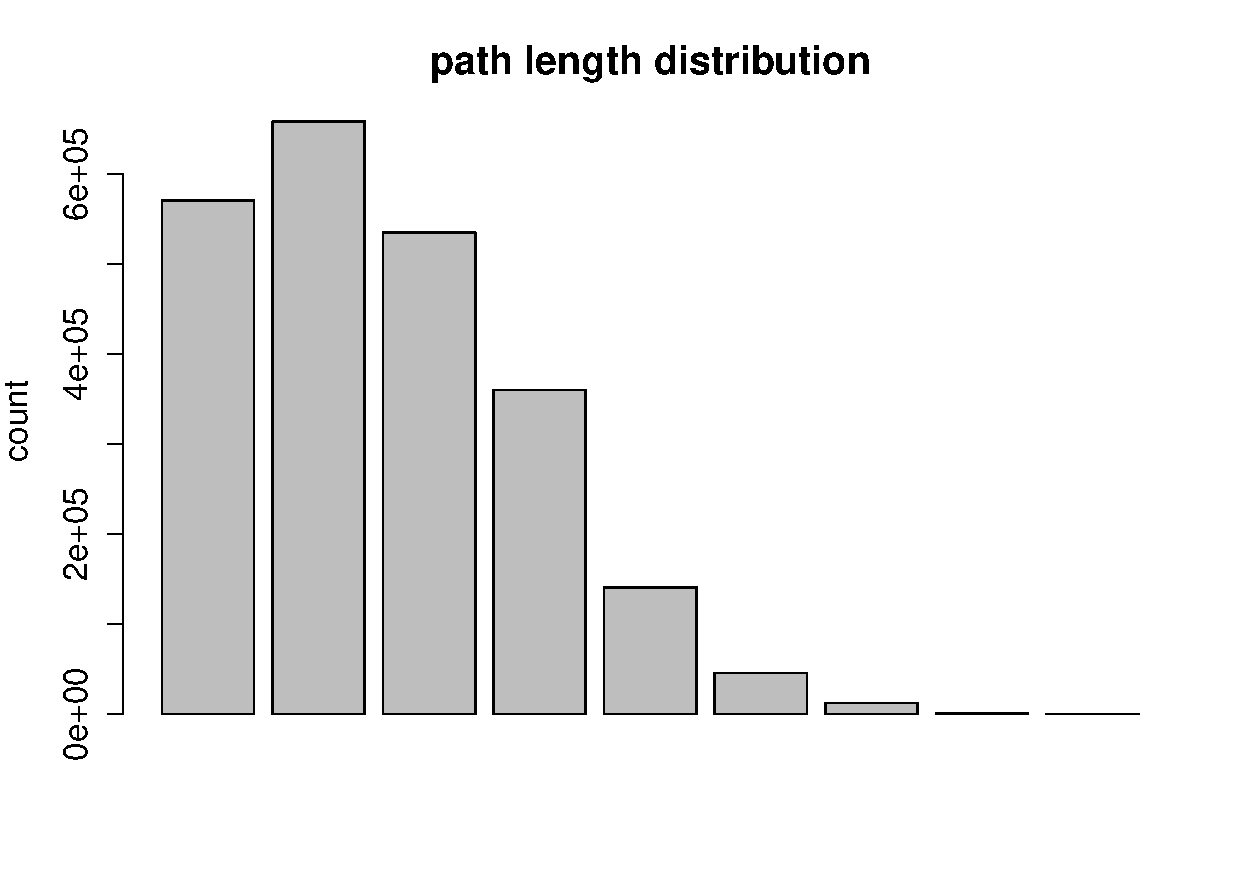
\includegraphics[width=0.5\textwidth]{figures/pathlength}
}


\jframe{Cliques(citation)}{
\vspace{-1cm}
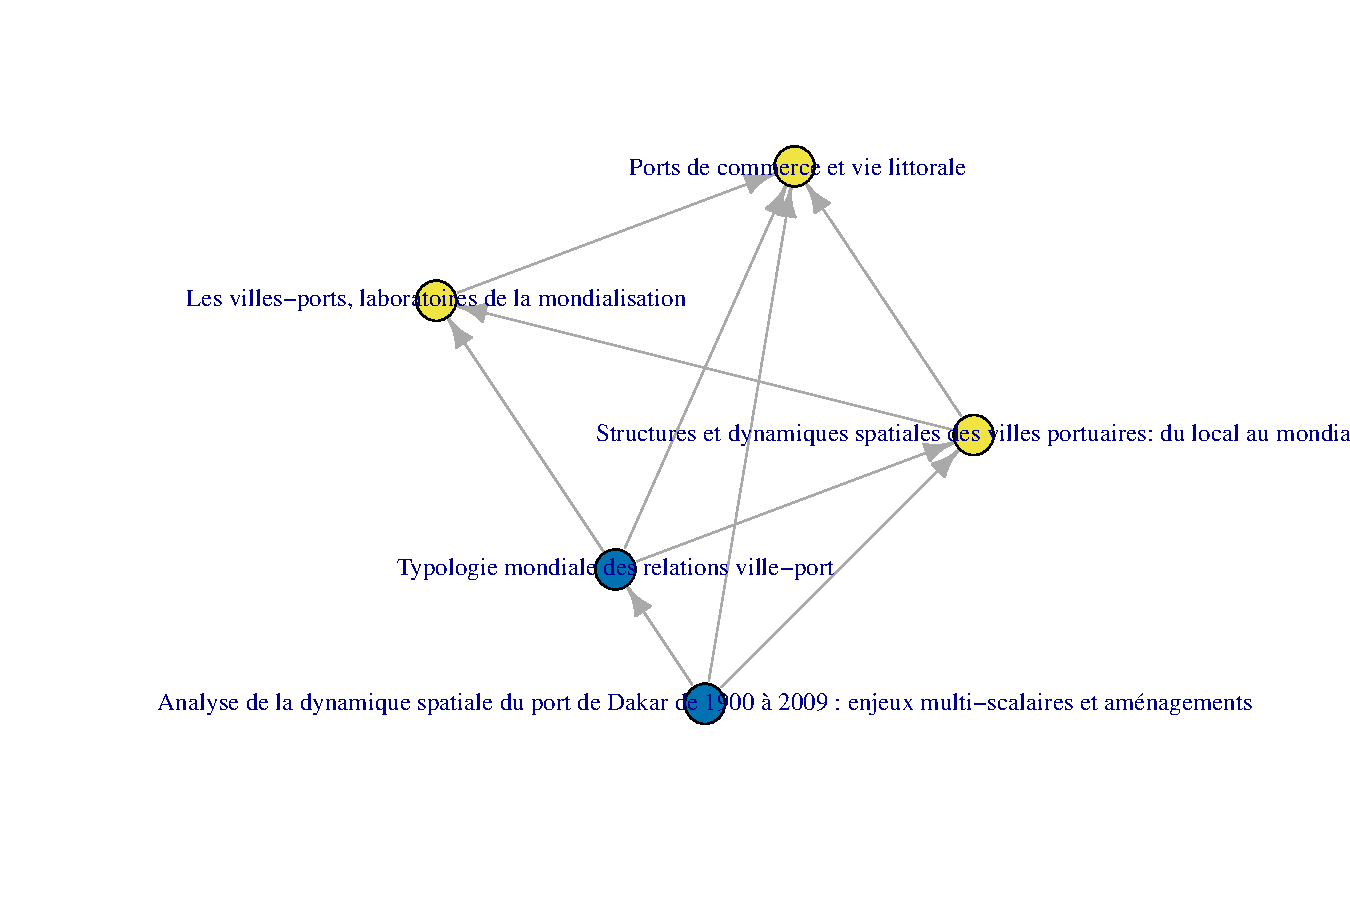
\includegraphics[height=\textheight]{figures/cybclic_2cyb_12817}

}



\jframe{Network Perturbation}{

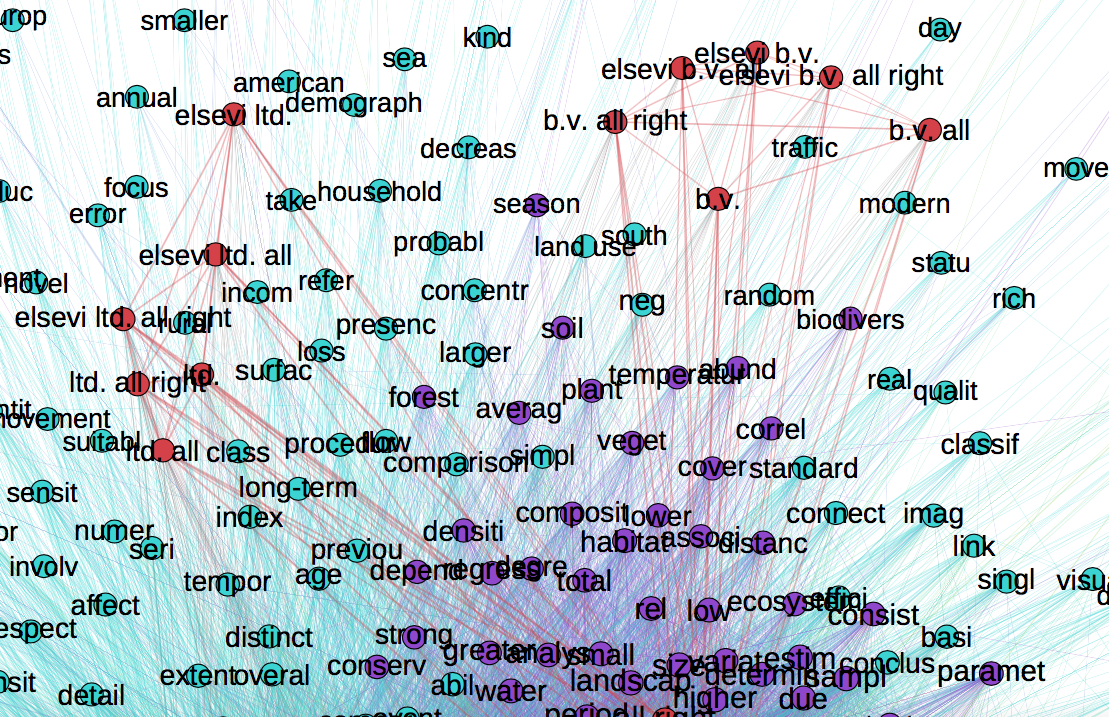
\includegraphics[height=\textheight]{figures/elsevierMotherFucker}

}




\jframe{Relevance estimation}{
Relevance estimation via statistical distribution of co-occurrences ($\chi^2$ score) : \textit{termhood} defined, with $M_{ij}$ number of articles where $i$ et $j$ appear simultaneously :
\[
t_i = \sum_{j\neq i}\frac{\left( M_{ij} - \sum_{k}M_{ik} \sum_{k} M_{jk}\right)^2}{\sum_{k}M_{ik} \sum_{k} M_{jk}}
\]


in $\Theta (\sum_i N_i^2)$ ($N_i$ abstract sizes) : difficult on a corpus where $\sum_i N_i^2 \simeq N <N_i>^2 \simeq 8\cdot 10^7$

}

\jframe{Relevance estimation}{

\textit{Bootstrap estimation tests (performance)}

\bigskip

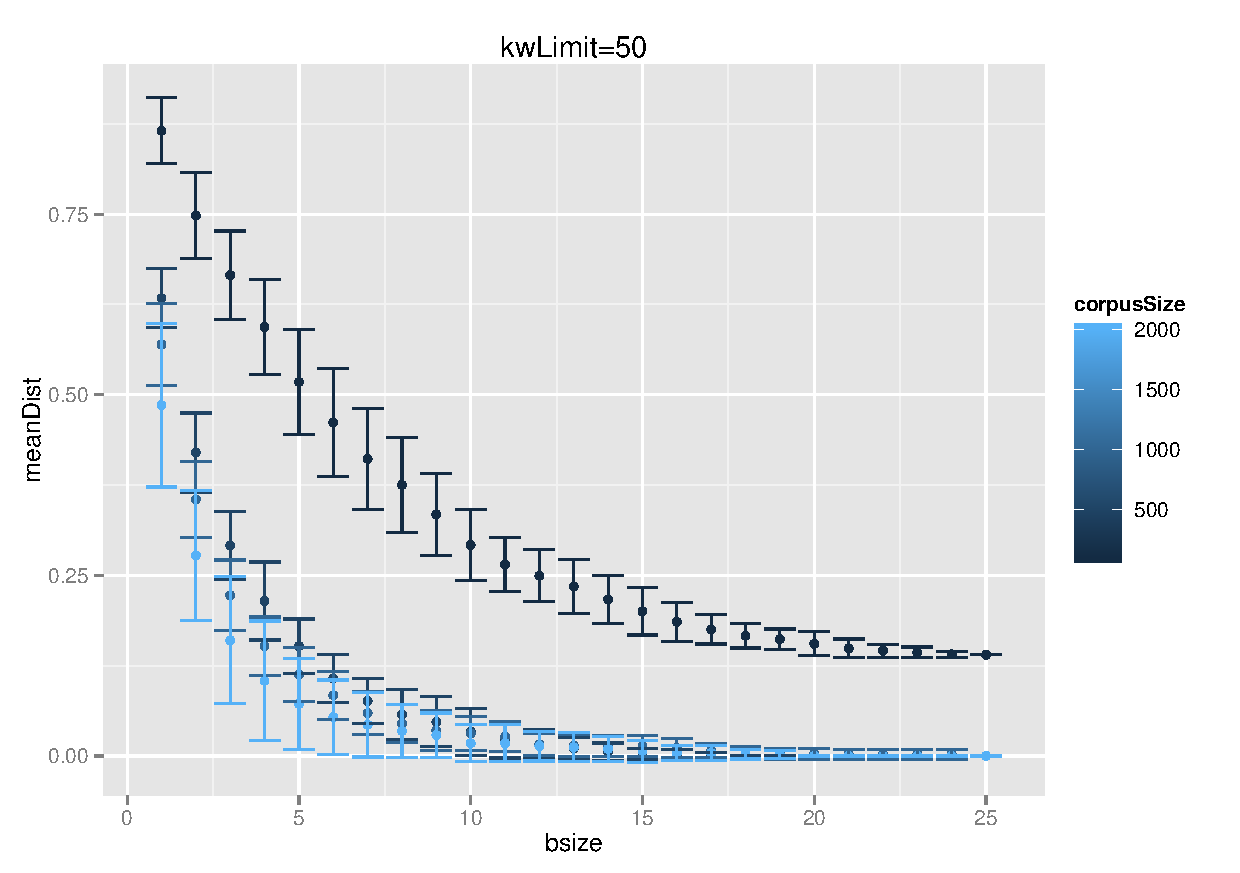
\includegraphics[width=0.5\textwidth]{figures/bootstrap_withReplacement_kw50}
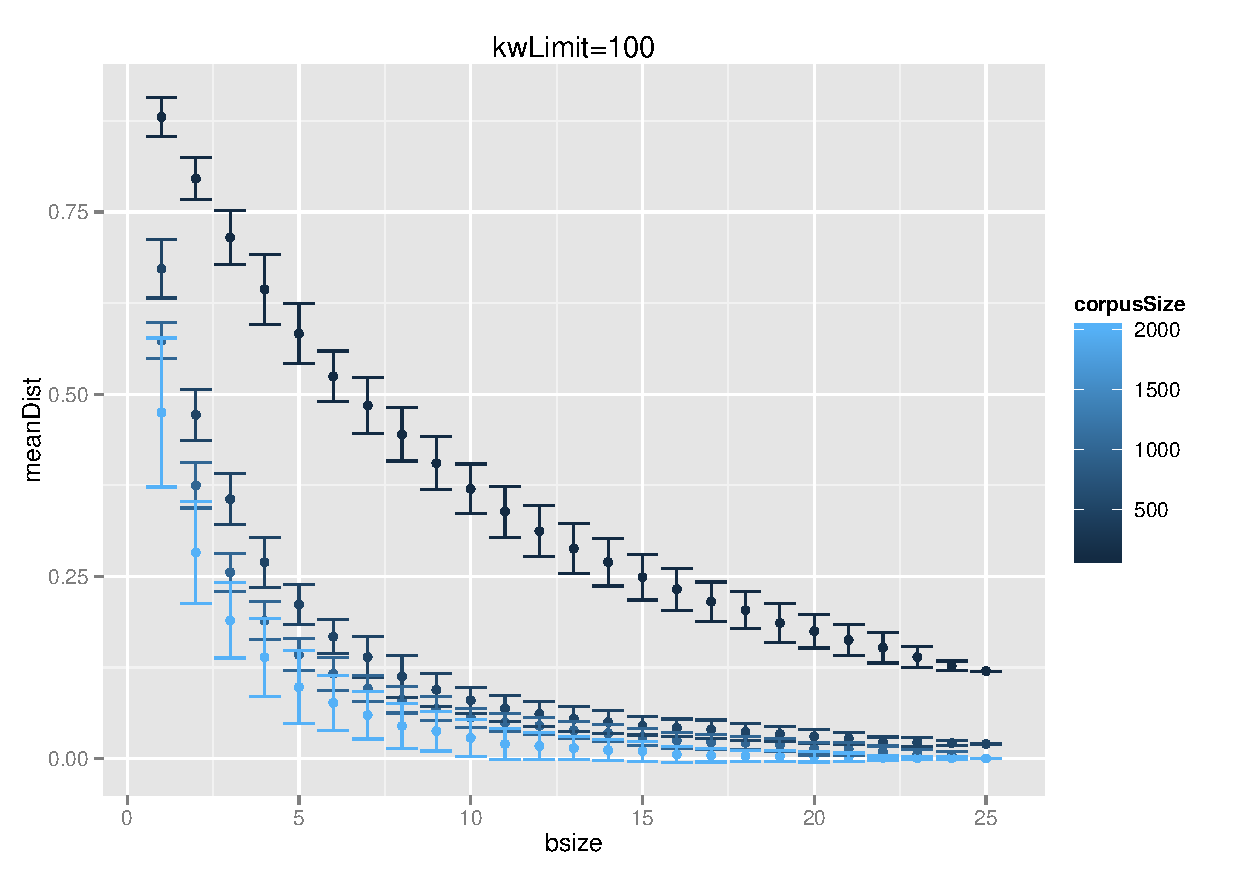
\includegraphics[width=0.5\textwidth]{figures/bootstrap_withReplacement_kw100}
}













%%%%%%%%%%%%%%%%%%%%%%%%%%%%%%%%
\begin{frame}[allowframebreaks]
\frametitle{References}
\bibliographystyle{apalike}
\bibliography{/Users/Juste/Documents/ComplexSystems/CityNetwork/Biblio/Bibtex/CityNetwork,/Users/Juste/Documents/ComplexSystems/CityNetwork/Docs/Papers/Cybergeo/Biblio/cybergeo,biblio}
\end{frame}
%%%%%%%%%%%%%%%%%%%%%%%%%%%%%%%%







\end{document}
